% Options for packages loaded elsewhere
\PassOptionsToPackage{unicode}{hyperref}
\PassOptionsToPackage{hyphens}{url}
%
\documentclass[
  12pt,
]{article}
\usepackage{amsmath,amssymb}
\usepackage{iftex}
\ifPDFTeX
  \usepackage[T1]{fontenc}
  \usepackage[utf8]{inputenc}
  \usepackage{textcomp} % provide euro and other symbols
\else % if luatex or xetex
  \usepackage{unicode-math} % this also loads fontspec
  \defaultfontfeatures{Scale=MatchLowercase}
  \defaultfontfeatures[\rmfamily]{Ligatures=TeX,Scale=1}
\fi
\usepackage{lmodern}
\ifPDFTeX\else
  % xetex/luatex font selection
\fi
% Use upquote if available, for straight quotes in verbatim environments
\IfFileExists{upquote.sty}{\usepackage{upquote}}{}
\IfFileExists{microtype.sty}{% use microtype if available
  \usepackage[]{microtype}
  \UseMicrotypeSet[protrusion]{basicmath} % disable protrusion for tt fonts
}{}
\makeatletter
\@ifundefined{KOMAClassName}{% if non-KOMA class
  \IfFileExists{parskip.sty}{%
    \usepackage{parskip}
  }{% else
    \setlength{\parindent}{0pt}
    \setlength{\parskip}{6pt plus 2pt minus 1pt}}
}{% if KOMA class
  \KOMAoptions{parskip=half}}
\makeatother
\usepackage{xcolor}
\usepackage[margin=1in]{geometry}
\usepackage{graphicx}
\makeatletter
\def\maxwidth{\ifdim\Gin@nat@width>\linewidth\linewidth\else\Gin@nat@width\fi}
\def\maxheight{\ifdim\Gin@nat@height>\textheight\textheight\else\Gin@nat@height\fi}
\makeatother
% Scale images if necessary, so that they will not overflow the page
% margins by default, and it is still possible to overwrite the defaults
% using explicit options in \includegraphics[width, height, ...]{}
\setkeys{Gin}{width=\maxwidth,height=\maxheight,keepaspectratio}
% Set default figure placement to htbp
\makeatletter
\def\fps@figure{htbp}
\makeatother
\setlength{\emergencystretch}{3em} % prevent overfull lines
\providecommand{\tightlist}{%
  \setlength{\itemsep}{0pt}\setlength{\parskip}{0pt}}
\setcounter{secnumdepth}{5}
\usepackage{setspace,lscape} \usepackage{amsmath} \usepackage{array} \usepackage{caption,subcaption,multirow} \usepackage[hang]{footmisc} \usepackage{enumitem} \usepackage{standalone} \renewcommand{\arraystretch}{1.5} \captionsetup[table]{skip=5pt} \setstretch{1.5} \setlength{\parindent}{1em} \setlength{\footnotemargin}{3mm} \setlength{\footnotesep}{3mm} \renewcommand{\[}{\begin{equation}} \renewcommand{\]}{\end{equation}}
\ifLuaTeX
  \usepackage{selnolig}  % disable illegal ligatures
\fi
\usepackage[]{natbib}
\bibliographystyle{apalike}
\IfFileExists{bookmark.sty}{\usepackage{bookmark}}{\usepackage{hyperref}}
\IfFileExists{xurl.sty}{\usepackage{xurl}}{} % add URL line breaks if available
\urlstyle{same}
\hypersetup{
  pdftitle={Attention and Valuation for Sequences of Rewards},
  pdfauthor={Zijian Zark Wang},
  hidelinks,
  pdfcreator={LaTeX via pandoc}}

\title{Attention and Valuation for Sequences of Rewards}
\author{Zijian Zark Wang}
\date{May 08, 2024}

\begin{document}
\maketitle
\begin{abstract}
(to be added)
\end{abstract}

\hypertarget{introduction}{%
\section{Introduction}\label{introduction}}

Attention is pivotal for people to make decisions in information-rich
environments. In everyday life, people often face economic decisions
that involve receiving rewards at different points in time. For
instance, to decide whether to invest in a pension plan, they have to
take into account the potential benefits they could receive at various
future times. Such decisions usually require people to calculate the
total value of multiple rewards, each with multiple attributes (time and
amount). Because of the variety of information involved, it is highly
likely that attention plays a key role in their decision processes.
However, there is a significant gap in research on how attention may
affect the valuation of reward sequences. In this paper, we explore this
topic with three pre-registered experiments.

To valuate a sequence of rewards, people may have to process the
information about each amount they could receive, and then bind it with
certain time information, and finally, aggregate them to obtain a
representation of total value. We borrow from the previous research
about attention and propose that attention plays a role in each stage of
this process. First, when they process an individual amount, they need
to extract certain information from their mind and use it as an evidence
to support their valuatation. Paying more attention to the amount may
facilitate the extraction of information and amplify its value. Relevant
literature includes drift-diffusion models
\{\citep[DDMs, see][]{ratcliff2016diffusion}) and query theory
\citep{weber2007asymmetric, johnson2007aspects}. In addition,
\citet{krajbich2010visual} import an attention parameter into DDMs to
capture this effect. Second, when people combine the amount and time
attributes, they may tend to focus on one attribute and ignore the
other. A relevant evidence is that consumers sometimes use the
``take-the-best'' heuristic \citep{gigerenzer2011heuristic} in
multi-attribute choices: taking into account only one attribute each
time and and making choices entirely based on that attribute. Third,
when they integrate the different information to construct an aggregate
value representation, they may tend to overweight the rewards with large
values and underweight (but still assign some weight to) the rewards
with small values, given the former attract more of their attention. The
relevant evidence include value-driven attentional
capture\citep{hickey2010reward, anderson2011value, chelazzi2013rewards}
and the hidden-zero effect
\citep{magen2008hidden, radu2011mechanism, read2017value}. The same
notion has been widely adopted by theories involving risky choices, such
as the salience theory \citep{bordalo2012salience, bordalo2013salience}
and utility-weighted sampling \citep{lieder2018overrepresentation}.

In three separate experiments, we investigated each of the three
channels through which attention operates. In each experiment, we set up
a simple choice context in which decision makers are asked to choose
between two options. Under one option, they can receive an amount \(M\)
immediately (e.g.~``receive £120 today''). Under the other option, they
can receive an amount \(X_1\) immediately and another amount \(X_T\) in
delay \(T\) (e.g.~``receive £80 today and £70 in 12 months''). The
latter option is called a ``sequence option'' and we investigate how
decision makers' preference for this option is affected by attention and
elements in that option.

In Experiment 1, we exogenously direct the decision makers' attention to
the delayed reward in the sequence option. We force the decision makers
to view the options before they are allowed to make a choice, and then
block out a part of each option. After they have made a choice, an
additional question appears on the same screen asking them the content
of the sequence option. The part being blocked contains the delayed
reward of the sequence option, so they have to answer the question in
the situation of having access to this relevant information. To
correctly answer the additional question, decision makers have to pay
special attention to the delayed reward during the forced viewing period
(when considering their choices). We find that this manipulation method
significantly increase their preference for the sequence option, which
indicates the value of the delayed reward might be amiplified by
attention. Moreover, we apply the same manipulation method to a
perceptual choice task (irrelevant to valuation) and find it has no
effect on choices. This experiment also provides a direct evidence on
how attention can affect intertemporal choices.

Experiment 2-3 investigate the role of attention by manipulating the
elements in the sequence option. In Experiment 2, we leave a blank for
the amount \(M\), and ask participants to identify which level of this
amount can make them indifferent between the two options. Suppose
decision makers are indifferent between the two options when \(M=Y\). We
find a substantial proportion of participants totally ignore the time
attribute in this task: their answers are simply the sum of two amounts
in the sequennce option, i.e.~\(Y=X_1+X_T\) (they do not consider any
delay discounting). These specific responses may be related to a
heuristic as they take less time than other responses.

For the remaining participants in Experiment 2, we find \(Y-X_1\) is
decreasing in \(X_1\), keeping the others equal. This behavioral pattern
significantly deviates from some widely-used discounted utility
theories. The discounted utility theories typically assume
\(u(Y)=u(X_1)+w_T\cdot u(X_T)\), where \(u(.)\) is a concave utility
function and \(w_T\) is a discount factor. Under certain \(T\) and
\(X_T\), \(u(Y)-u(X_1)\) should be constant. Because \(u(.)\) is
concave, each increase in \(X_1\) should incur a larger increase in
\(Y\). So, this implies that \(Y - X_1\) is increasing in \(X_1\) (note
\(Y\) could be decomposed to \(Y-X_1\) and \(X_1\)), which is opposite
to our finding.

The behavioral pattern that \(Y-X_1\) decreases with \(X_1\), as well as
the results of Experiment 3, can provide an implication for modifying
the discounted utility theories. Note \(X_1\) is a common amount in both
options. Thus, \(Y-X_1\) reflects the present value of the delayed
reward. Our finding suggests increasing the immediate reward \(X_1\) in
the sequence option could make the value of delayed reward more
discounted. In Experiment 3, we investigate the interactions between the
values of different rewards in the sequence option with another
approach: participants are asked to make a series of choices under
different \(M\), \(X_1\), \(X_T\) and \(T\) (elements in those options).
We infer the indifference points bewteen options through these choices.
We find that, keeping the others equal, under a larger \(X_1\), their
indifference points characterized by \(X_T\) exhibit a greater
randomity. Meanwhile, under a larger \(X_T\), their indifference points
characterized by \(X_1\) also exhibit a greater randomity. We estimate
the implication of these results for the discounted utility theories by
estimating a probabilistic choice model. The model estimation results
suggest that increasing the amount of one reward (either \(X_1\) or
\(X_T\)) could make the value of the other reward more discounted. In
other words, people tend to underweight a small reward when there is a
large reward in the sequence.

Moreover, in Experiment 3, we also find that under a larger sequence
length \(T\), the participants' indifference points characterized by
\(X_1\) exhibit a greater randomity. Within the discounted utility
framework, this could indicate that the value of the immediate reward is
more discounted when the immediate reward and the delayed reward in the
same sequence are far away from each other (there are more zero values
between them). This result is consistent with the hidden zero effect. To
our knowledge, the result is not captured by most of the existing
discounted utility theories. We propose that one method to incorporate
this in discounted utility is to assume that the total capacity of
weights (discount factors) that a decision maker can allocate across
different time points is fixed at some certain level.

The remainder of this paper is organized as follows. Section 2 discusses
the possible channels through with attention can affect the valuation of
reward sequences. Section 3 presents the implications of overweighting
(underweighting) certain values within the discounted utility framework.
Section 4-6 presents the each experiments. Section 6 discusses the
relationship between our experimental results and the existing theories
about time discounting.

\hypertarget{how-attention-may-shape-the-value-of-a-reward-sequence}{%
\section{How Attention May Shape the Value of A Reward
Sequence}\label{how-attention-may-shape-the-value-of-a-reward-sequence}}

\hypertarget{elemental-properties-of-attention}{%
\subsection{Elemental Properties of
Attention}\label{elemental-properties-of-attention}}

There is currently no consensus among scholars on what attention is.
However, many scholars have acknowledged that attention is constituted
by multiple cognitive mechanisms, and identified some of its elemental
properties. Here we present four properties of attention on which our
research is grounded.

First, attention is selective. Back in \citeyear{james1890}, William
James described the underlying principle of attention as ``withdrawal
from some things in order to deal effectively with others''. Since then,
various studies have suggested attention has the function of filtering
certain information into consciousness (or inhibiting the processing of
other information) when people are overloaded with information. A more
modern view, proposed by \citet{gottlieb2010attention},
\citet{gottlieb2012attention} and \citet{sharot2020people}, describes
attention as an active sampler, making selections based on the utility
of information. These scholars summarize a range of neuroscientific
evidence and state that people tend to pay attention to information with
higher instrumental utility (reducing uncertainty), hedonic utility
(associated with a significant reward), or cognitive utility (satisfying
curiosity).

Second, attention is the allocation of limited capacity. This capacity
view of attention was firstly proposed by \citet{kahneman1973}.
According to Kahneman's view, processing information consumes cognitive
resources in the brain, therefore people need attention to allocate
their limited cognitive resources to different information sources.

Third, attention could be driven by both exogenous factors and
endogenous factors. These factors drive attention through various ways.
A salient stimuli which is exogenous, can naturally capture attention,
whereas a goal which is endogenous, can alter attention through
consuming cognitive resources. Notably, recent research suggests an
endogenous factor can also capture attention
\citep{awh2012top, failing2018selection}. A typical example is
``\emph{value-driven attentional
capture}''\citep{hickey2010reward, anderson2011value, chelazzi2013rewards}.
In relevant studies, researchers ask people to do a series of visual
search tasks, and in each task, people can get a reward for detecting a
target object from distractors. The value-driven attentional capture
effect implies that an object associated with large rewards in preceding
tasks can capture participants' attention. Therefore, when it is being a
distractor, it can naturally slow down the target detection.

Fourth, attention is decisive for people to resolve objects, and to
scrutinize and recognize their features and actions
\citep{he1996attentional, intriligator2001spatial}. Figure
\ref{fig:attention_example} demonstrates the role of attention in this
respect with a simple example. Many scholars use ``spotlight'' as a
metaphor for attention. For areas illuminated by the spotlight, people
can easily discern any changes occurring within. But for areas outside
of the spotlight, they may not be sensitive to changes happening there.

\begin{figure}   
  \vspace{16pt}   
  \centering   
  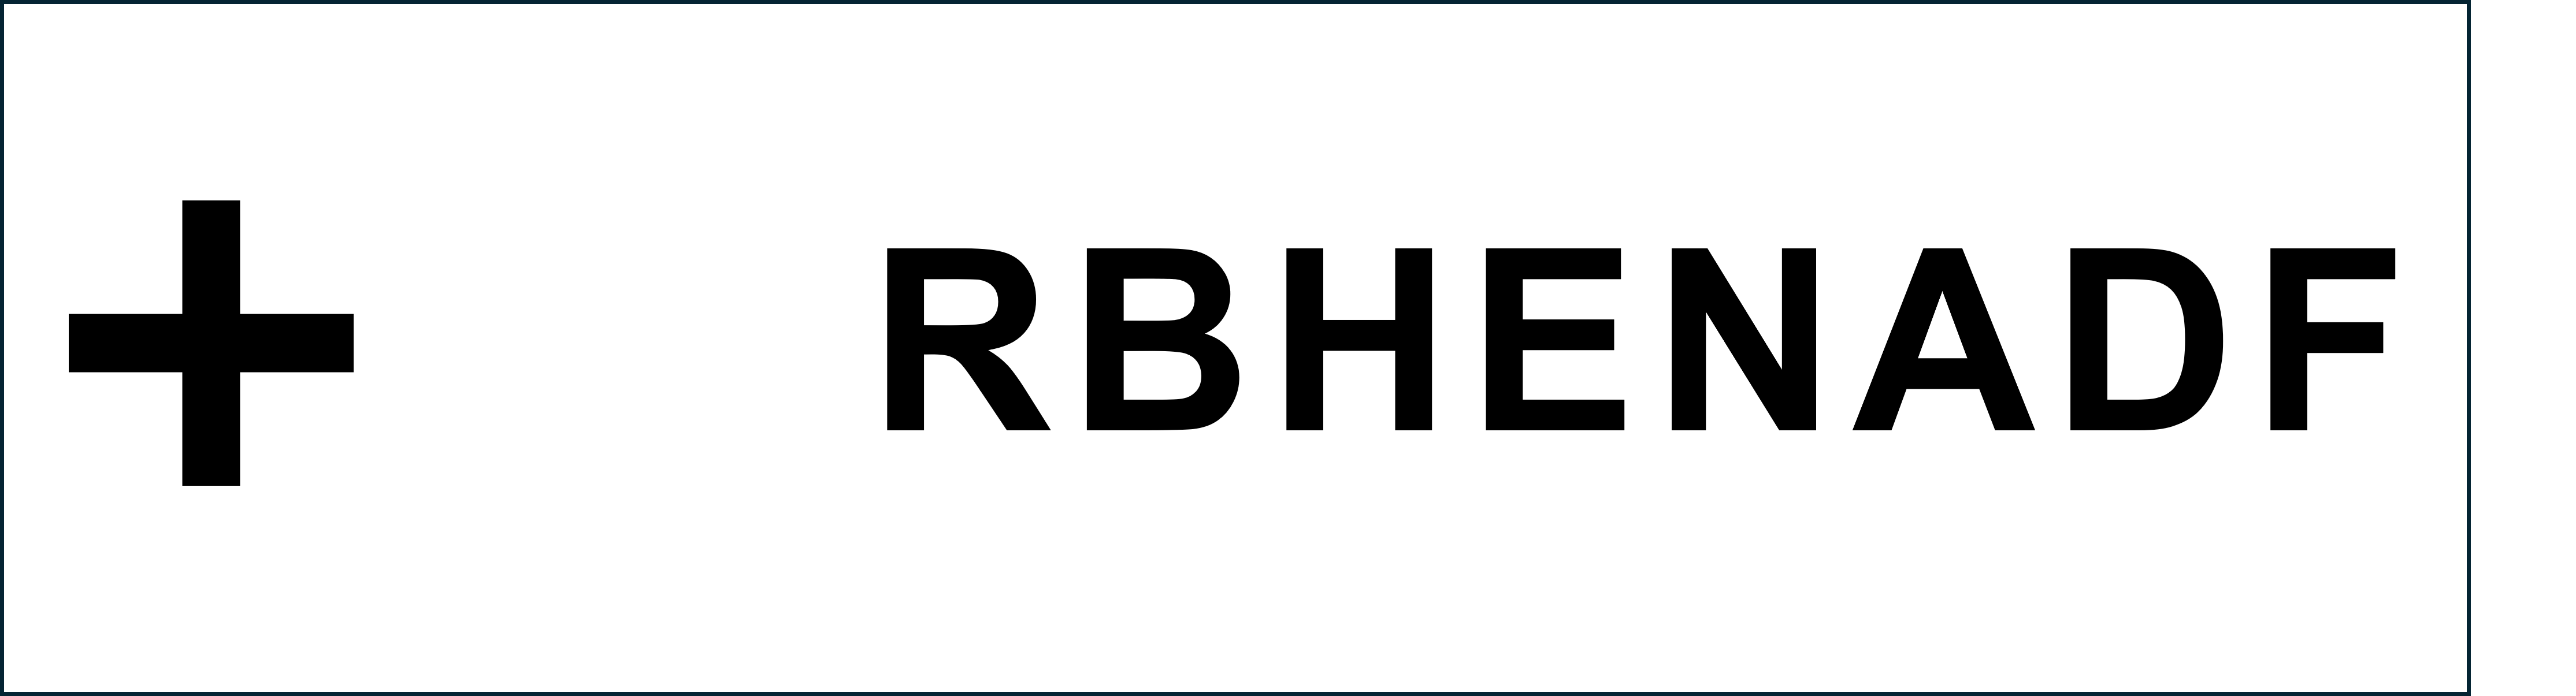
\includegraphics[width=0.96\textwidth]{figures/attention_example.png}    
  \caption{The role of attention in resolving objects}   
  \label{fig:attention_example}

\vspace*{4pt}  
\begin{minipage}{1.0\textwidth}
{\par\footnotesize Note: Keep your eyes around 30cm away from the page, and fixate the cross. The letters to the right are easily seen. However, it may be difficult to identify what the fifth letter is (``\textbf{N}'') because few attention is paid to it.}
\end{minipage}  
\end{figure}

\hypertarget{attention-enhances-values-for-individual-rewards}{%
\subsection{\texorpdfstring{Attention Enhances Values for Individual
Rewards
\label{attention_value}}{Attention Enhances Values for Individual Rewards }}\label{attention-enhances-values-for-individual-rewards}}

There is a growing body of literature suggesting, when people face a
choice between multiple rewards, directing their attention to one reward
(or the positive aspects of it) can increase its value.\footnote{\citet{orquin2013attention}
  reviewed some relevant evidence. For more recent studies, see
  \citet{smith2019gaze}, \citet{gwinn2019spillover} and
  \citet{pleskac2023attention}. For studies in the field of
  intertemporal choices, see \citet{franco2016now} and
  \citet{fisher2021intertemporal}. Also, note all rewards in this paper
  refer to positive rewards (gains rather than losses).} A theoretical
explanation involves viewing the valuation of a certain reward as an
evidence-accumulation process. When decision makers selectively spend
more cognitive resources processing a positive reward, they may be able
to accumulate a greater amount of evidence to support their preference
for it, thereby increasing its value. Or, if they selectively prioritize
the processing of positive evidence toward a reward, it may inhibit the
processing of the negative evidence that emerges subsequently, which
also increases its value.

Examining the causal effect of attention on reward valuation involves
exogeneously manipulating the drivers of attention in experimental
settings. In existing studies, there are two typical attention
manipulation methods. The first is through controlling the gaze
duration, such as presenting rewards in order and each with certain
duration
\citep{shimojo2003gaze, armel2008biasing, fisher2021intertemporal, bhatnagar2022meta}.
The second is to prioritize the processing of certain information. For
example, one can increase visual saliency of an option
\citep{milosavljevic2012relative}, or ask participants to fixate a
certain area around the option when making choices
\citep{lim2011decision}, to let them prioritize the perceptual
processing of that option. Besides, in a choice task,
\citet{weber2007asymmetric} ask people to think about the positive
aspects of an option first and then the negative aspects, and list their
thoughts. This manipulation prioritizes the processing of certain
semantic information. In a review, \citet{mormann2021does} argue that
gaze duration is not identical to attention. Thus, we design our study
with the second method.

Most studies on causal relationship between attention and value are set
up with two options, and each option contains only one reward. So far,
the only study investigating this topic in the intertemporal choice
field is \citet{fisher2021intertemporal}. In that study, participants
are presented with a small-sooner reward (SS) and a large-later reward
(LL), and the researcher finds directing their attention to one reward
can increase the preference for it. In our Experiment 1, we investigate
whether we can apply a similar result to the case where an option is a
sequence of multiple rewards. To illustrate, imagine that you face a
choice between:

\setlength{\leftskip}{24pt}

A. receive £200 today

B. receive £100 today and £130 in 6 months

\setlength{\leftskip}{0pt}

Taking receiving £100 today as the benchmark. By choosing option A, you
can get an additional amount of £100 today; by choosing option B, you
can get an additional amount of £130 in 6 months later. So, the choice
is similar with a choice between SS and LL. Suppose before you make the
decision, we direct your attention to the second reward in option B,
i.e.~receiving £130 in 6 months. Then, your preference for option B may
increase, because it is the same as directing your attention to a LL. To
test this hypothesis, in Experiment 1, we design a novel attention
manipulation method which let participants to prioritize the semantic
processing of that reward. We find this method can effectively alter
participants' preferences in our experimental context.

\hypertarget{inattention-to-time-attribute}{%
\subsection{\texorpdfstring{Inattention to Time Attribute
\label{attention_time}}{Inattention to Time Attribute }}\label{inattention-to-time-attribute}}

When people face a choice between SS and LL, some may make comparisons
between attributes (time and amount) while others may make comparisons
between rewards. For instance, in one study, \citet{reeck2017search}
cluster participants into two groups using their mouse trajectories
during the decision process. About half of the participants tend to
switch mouse between attributes and the other half tend to switch mouse
between options. The former may indicate attribute-wise comparison while
the latter may indicate option-wise comparison.

One study of \citet{fisher2021intertemporal} investigates how allocating
attention across attributes may affect the choice between SS and LL. The
researcher finds that directing participants' attention to the time
attribute can increase their preference for SS while to the amount
attribute can increase their preference for LL. However, in a choice
involving sequences, focusing on one attribute and ignoring the other
could have a different implication for decision making. As an
illustration, imagine that you have two options:

\setlength{\leftskip}{24pt}

C. receive £100 today and £70 in 6 months

D. receive \_\_\_\_\_ today

\setlength{\leftskip}{0pt}

and you can fill in the blank in option C with any amount. Then, with
what amount, you would become indifferent between the two options? The
answer will depend on how you value each option. Suppose you think about
each attribute separately. In terms of the amount attribute, option C
contains two amounts, £100 and £70. In terms of the time attribute,
option C contains two dates when you can receive a positive reward,
``today'' and ``6 months later''. Since the question asks you to fill in
an amount, focusing on amounts and ignoring the times may be more nature
than the opposite. In an extreme case, if you totally ignore the time
attribute, then the times should have no impact on your valuation, so
the amount you fill should be exactly the sum of two amounts in option
C. In Experiment 2, we find a supportive evidence for this. Notably,
this causes their behavior to deviate from any prediction made through
time discounting theories.

\hypertarget{in-attention-to-small-values}{%
\subsection{\texorpdfstring{(In-)attention to Small Values
\label{attention_small}}{(In-)attention to Small Values }}\label{in-attention-to-small-values}}

Now suppose a decision maker valuates a reward sequence by valuing each
reward (rather than each attribute) separately and then binding the
values together. In Section \ref{attention_value}, we discuss how
attention may affect the value of each individual reward. Here we
discuss how attention may affect the process of binding values together.

Our discussion is primarily driven by the evidence of \emph{value-driven
attention capture} and the \emph{hidden-zero effect}. The value-driven
attentional capture implies objects with large values can capture
people's attention, particularly in visual search. We propose the same
remark could apply to the valuation of reward sequences. Once a reward
is associated with a large value, it also captures attention and thus,
given attention is limited, people become inattentive to other (small)
rewards in the sequence. As a result, they may take more into account
the large rewards and less into account the small rewards during their
valuation of the sequence.

Consider the choice between option C and option D again. Suppose the
earlier amount in option C is increased from £100 to £1,000, so that the
option becomes ``receive £1,000 today and £70 in 6 months''. Then, when
a decision maker is valuing this option, the earlier amount £1,000 can
capture more of her attention and the later amount £70 could be
relatively ignored. In the original case, she may value option C equally
as much as ``receive £160 today'', which implies the present value of
the later amount is equal to £60. But in the case that the earlier
amount is increased to £1,000, whether she can get an additional amount
of £70 in 6 months later is less important, so the present value of the
later amount could decrease to some smaller number (say, equal to £20).
Under this circumstance, she may value option C equally as much as
``receive £1,020 today''. Moreover, since she ignores the later amount,
she would be insensitive to the changes in that while valuating the
sequence. In other words, any change in the later amount should lead to
a smaller change in the total value of sequence.

The hidden-zero effect \citep{magen2008hidden, radu2011mechanism}
implies when decision makers valuate a reward sequence, they also take
into account the value of zero rewards. \citet{read2017value} find the
hidden-zero effect is asymmetric. To illustrate, suppose people are
indifferent between ``receive £100 now'' (SS), and ``receive £120 in 1
year'' (LL). The (asymmetric) hidden-zero effect indicates, keeping the
others equal, changing SS to ``receive £100 now and £0 in 1 year'' would
make people more likely to choose LL, whereas changing LL to ``receive
£0 now and £120 in 1 year'' has no effect on their preferences. An
explanation is that people perceive the original SS as a single
immediate reward (or a very short sequence) and the original LL as a
sequence delivering zero reward at any time within a year. Specifying
the zero amount for SS triggers people to notice there are zero rewards
delivered in the far future, which they originally did not consider.
Given their attention is limited, this may reduce their attention to the
immediate reward £100. As a result, they take less into account the
amount £100 and more into account zeros which they will receive in the
future, thereby devaluing the SS. By contrast, when valuing the LL, they
have already taken those zeros into account, so specifying the zero
amount has no effect on their preferences for LL.

In the case that a decision maker can ``receive £100 today and £70 in 6
months'', the hidden-zero effect has another implication. If we increase
the delay ``6 months'' to ``12 months'', there will be more zeros being
considered in this sequence and thus the attention assigned to both the
earlier and later amounts should decrease. On the one hand, this should
decreases the total value of sequence. On the other hand, the total
value should be less sensitive to not only the changes in the later
amount, but also the changes in the earlier amount.

\hypertarget{implications-of-attention-to-small-values-for-time-discounting}{%
\section{Implications of Attention to Small Values for Time
Discounting}\label{implications-of-attention-to-small-values-for-time-discounting}}

\hypertarget{theoretical-background}{%
\subsection{Theoretical Background}\label{theoretical-background}}

We restate the arguments about (in-)attention to small values in Section
\ref{attention_small} with a more formal framework. Consider a decision
maker facing a choice between two options. Under one option, she could
receive \(X_1\) now and \(X_T\) in delay \(T\); under the other option,
she could receive \(M\) now and no reward at any other times (\(X_1\),
\(X_T\), \(T\), and \(M>0\)). According to the additive discounted
utility theories, the value of the former option can be represented by
\(w_1\cdot u(X_1) +w_2\cdot u(X_T)\) and that of the latter option can
be represented by \(k\cdot u(M)\), where \(u(.)\) is a strictly
increasing and strictly concave utility function, and \(u(0)=0\). The
parameters \(w_1\), \(w_T\), \(k\) are the weights (somtimes called
discount factors) assigned to \(X_1\), \(X_T\) and \(M\) in each option.
Hereafter, we call the first option a ``sequence option'', and the
second option a ``single option''. In a sequence option, the amount
delivered immediately is called the ``\emph{front-end amount}'', and the
amount delivered later is called the ``\emph{back-end amount}''.

In the sequence option, one unit change in \(u(X_t)\) will yield a
\(w_t\) unit change in the total value (\(t\in\{1,T\}\)). So, the weight
\(w_t\) somehow reflects decision makers' sensitivity to changes in
\(u(X_t)\) in terms of valuating the certain sequence. In Section
\ref{attention_small}, we propose that paying less attention to
\(u(X_t)\) would make decision makers less sensitive to it, thereby
decreasing \(w_t\). Furthermore, there are two situations that can alter
the volume of attention allocated to \(u(X_t)\). The first is that the
amount of another reward is increased by a sizeable level (value-driven
attentional capture). The second is that we add a tiny value, e.g.
\(u(0)\), to some time point after \(t\), but still in the sequence
(hidden-zero effect). In either situation, decision makers' attention
would be directed to somewhere other than the reward \(X_t\) and \(w_t\)
should decrease.

A widely adopted assumption about time discounting is that the weights
depend only on times. Several popular discounting theories, e.g.
exponential and hyperbolic discounting, have adopted this assumption.
However, our consideration about attention to small values predicts an
interaction between the weights and reward amounts. Moreover, we predict
the weight assigned to the current time, i.e.~\(w_1\), can also be
discounted, and can be discounted more when there is a large \(T\) or
\(X_T\). In the following two subsections, we analyze what particular
behavior, if being observed, will allow us to identify such an
interaction.

\hypertarget{implication-for-indifference-points}{%
\subsection{\texorpdfstring{Implication for Indifference Points
\label{impli_indiff_point}}{Implication for Indifference Points }}\label{implication-for-indifference-points}}

Suppose the decision maker is indifferent between the two options when
\(M=Y\). We call \(Y\) the ``indifference point'' in this context. In
the additive discounted utility framework, we have
\[ k\cdot u(Y) = w_1 \cdot u(X_1) + w_T \cdot u(X_T) \]Assume all the
weights depend only on times. In the given context, it implies we can
set \(k= w_1= 1\). Let both \(T\) and \(X_T\) be constant, then under
this assumption, \(w_T\cdot u(X_T)\) should also be constant. Thus, to
make Equation (1) hold true, \(u(Y) - u(X_1)\) should be constant. Given
that \(u(.)\) is strictly concave, for any positive number \(\Delta\),
we have \(u(Y+\Delta) - u(X_1 + \Delta) < u(Y) - u(X_1)\). We can
decompose \(Y\) by \(Y = X_1+(Y -X_1)\). If \(X_1\) is increased by
\(\Delta\) units, to make the equation hold true, \(Y\) should be
increased by an amount larger than \(\Delta\). That is, if the weights
depend only on times, \(Y - X_1\) should always increase with \(X_1\).

In reverse, under certain \(T\) and \(X_T\), if \(Y-X_1\) decreases with
\(X_1\), there must be an interaction between weights and amounts when
applying the additive discounted utility framework. We test this in
Experiment 2.

\hypertarget{implication-for-probabilistic-choices}{%
\subsection{\texorpdfstring{Implication for Probabilistic Choices
\label{impli_prob_choice}}{Implication for Probabilistic Choices }}\label{implication-for-probabilistic-choices}}

Consider the choice between the two options in a probabilistic choice
framework. Keeping the others equal, when either \(X_1\) or \(X_T\)
increases, decision makers would be more likely to choose the sequence
option. Let \(P\) denote the choice probability for the sequence option.
It is usually assumed that \(P\) is determined by the difference in
utility between options. Therefore,\[
P = \phi(w_1\cdot u(X_1)+w_T\cdot u(X_T)-k\cdot u(M)) 
\]where \(\phi:R\rightarrow [0,1]\) is a link function. We assume
\(\phi(.)\) is strictly increasing. When \(w_1\) is smaller, for each
unit increase in \(u(X_1)\), there should be a smaller increase in
\(P\). In this case, the choices of the decision maker tends to appear
more random. The same behavioral implication can apply to \(w_T\).

Keeping the others equal, if the weights depend only on times, then
\(w_1\) and \(w_2\) should be independent of \(X_1\), \(X_T\) and \(T\).
The attention to small values, as we stated in Section
\ref{attention_small}, has two implications to these weights. First,
based on value-driven attentional capture, we state a larger \(X_1\) may
reduce \(w_T\) and a larger \(X_T\) may reduce \(w_1\). Second, based on
the hidden-zero effect, we state a longer \(T\) may reduce not just
\(w_T\) but also \(w_1\). We test these implications in Experiment 3 by
estimating a specification of Equation (2) and see whether there is an
interaction between weights and different variables.

In summary, if people are (in-)attention to small values when valuating
a reward sequence, changing the delay or amount of one reward would not
just affect the weight assigned to itself, but should also interfere the
weight assigned to the another reward within the sequence. Our
Experiment 2-3 provide evidence for this.

\hypertarget{experiment-1-causal-manipulation-of-attention}{%
\section{Experiment 1: Causal Manipulation of
Attention}\label{experiment-1-causal-manipulation-of-attention}}

\hypertarget{design}{%
\subsection{Design}\label{design}}

Experiment 1 aims to test whether directing people's attention to a
reward can make them value that more, in the context of valuating reward
sequences. We set up a series of choice tasks. The tasks are divided
into four parts. Each task in Part 1-2 is called an intertemporal choice
task. Each task in Part 3-4 is called a count-the-rabbits task. At each
time there is only one task presented on the screen. The task screens
are developed with HTML and Javascript, and we deploy the experiment
through JATOS \citep{lange2015just}. Before each part begins, there are
2-3 example tasks to help participants get familiarized with the tasks
in the corresponding part.

In Part 1-2, each task contains two options. The first option, presented
on the top, is a single immediate monetary reward. The second option,
presented on the bottom, is a sequence of two positive monetary rewards:
one delivered immediately and the other delivered in some delay.
Participants are required to choose the option they prefer. When each
task begins, both options are not visible. Participants have to click a
``Display'' button to view the options. They are forced to view the
options for at least 1.8s (during this time, their mouse pointer will be
hidden) before they are able to make a choice.

In Part 1, after participants submit a choice, they can directly start
the next task. In Part 2, after submitting a choice, an additional
question will appear on the same screen. This additional question has
three options, and participants have to identify which one among the
three options is the sequence option for the current task. We inform
participants that the additional question is to test their understanding
and attention to the choice task, and ask them to try their best to
correctly answer this question. We name any task followed by such an
additional question as a task in the ``question'' part, and any task
without such a question as a task in the ``no question'' part. Figure
\ref{fig:exp3_screenshot}(a) demonstrates an example intertemporal
choice task.

Tasks in Part 3 follow the same format as in Part 1, while tasks in Part
4 follow the same format as in Part 2. Nevertheless, in Part 3-4 we
replace the monetary rewards by some rabbit symbols. In each
count-the-rabbits task, we have one option containing a single set of
rabbit symbols, and another option containing two sets of rabbit
symbols. Participants need to identify which option has more
``rabbits''. In Part 3, participants can directly move to the next task
once finishing the choice; In Part 4, following each choice, there is an
additional question asking them the exact number of rabbits in the
sequence option. Figure \ref{fig:exp3_screenshot}(b) demonstrates an
example count-the-rabbits task.\footnote{Given the format of
  count-the-rabbits tasks are the same as intertemporal choice tasks, in
  Figure \ref{fig:exp3_screenshot}(b), we only demonstrate the screen
  that the participants face when being asked tp making a choice.}

Participants are randomly assigned to two groups. In one group, in each
task once both options become visible, they remain visible until the
participants move to the next task. We call this group the
``full-exposure'' group (control group). In the other group, after both
options have been displayed for 1.8s, the right half of each option will
be blocked out. The participants need to make choices in the case that
only part of the information is visible (see Figure
\ref{fig:exp3_screenshot}). We call this second group the
``limit-exposure'' group (treatment group). Notably, since each option
has a different length of content, only in the sequence option will a
part of the information be actually blocked out. For the single option,
we only block out a blank space. In an intertemporal choice task, the
information being blocked is the delayed reward in the sequence option;
in a count-the-rabbit task, the information being blocked is the second
set of the rabbit symbols in the sequence option.

\begin{figure}
  \centering
  \begin{subfigure}{\textwidth}
    \centering
    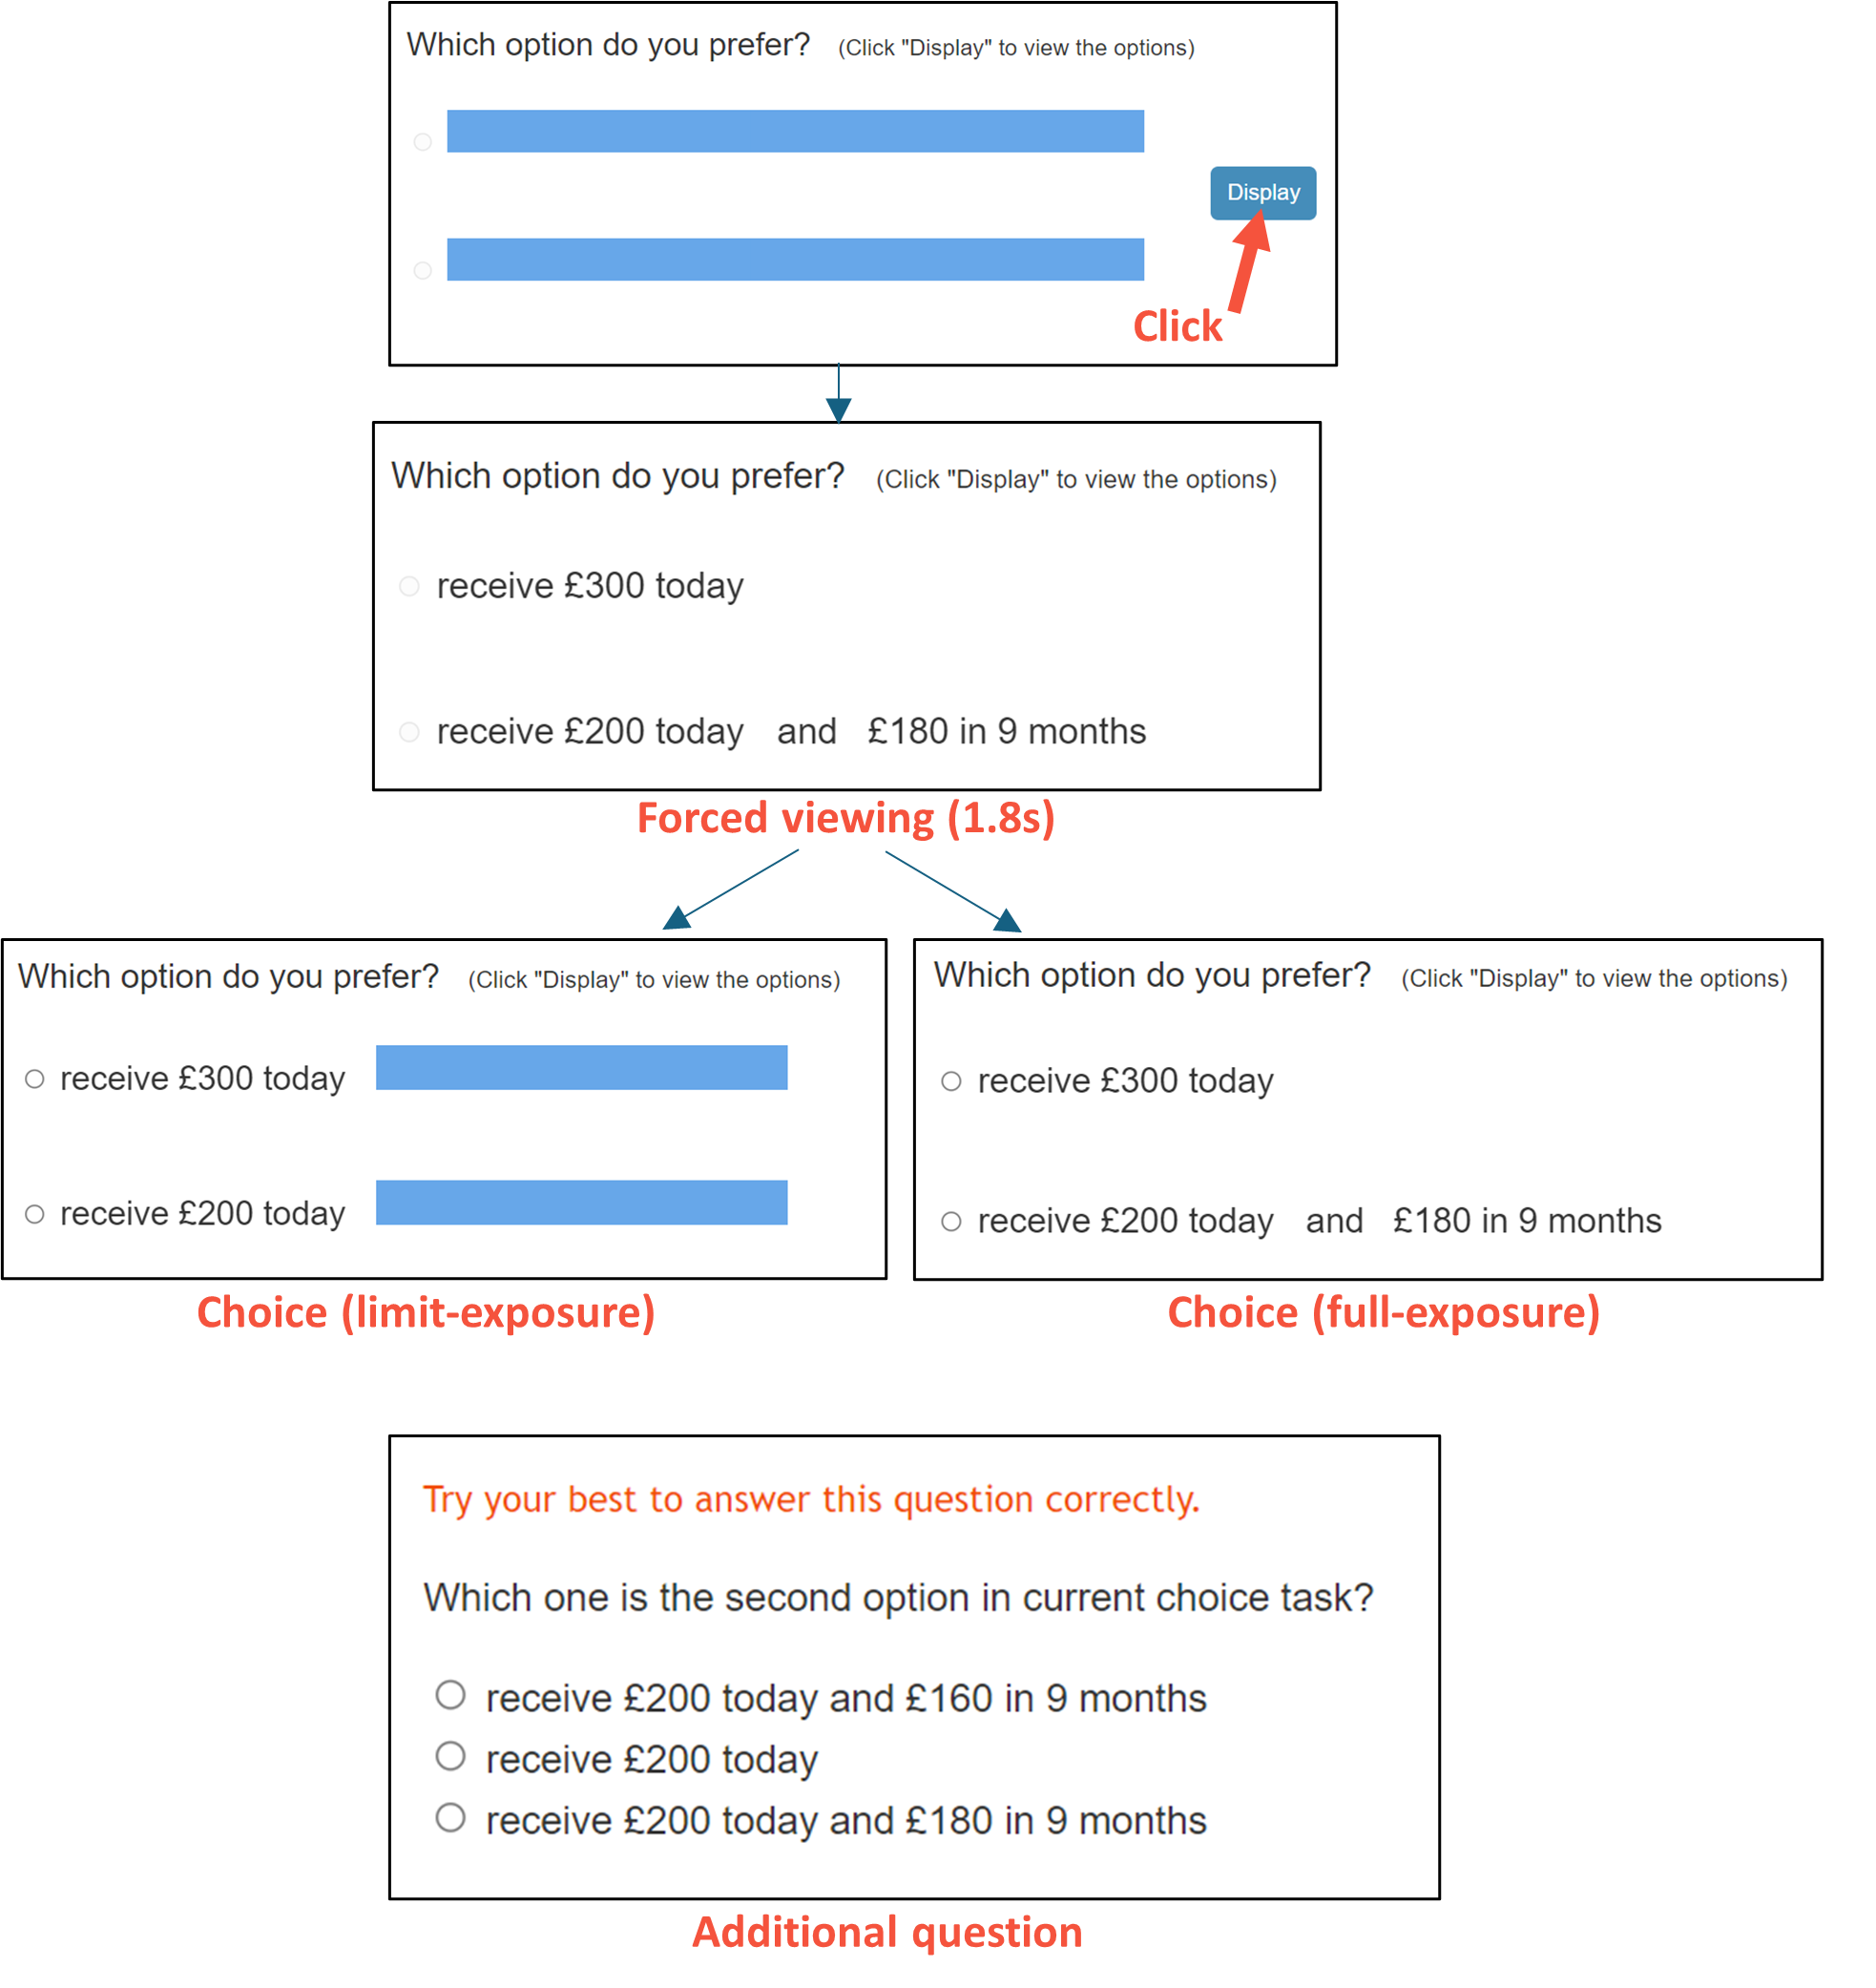
\includegraphics[width=\linewidth]{figures/exp3_screenshot_intertemporal.png}
    \subcaption{Intertemporal Choice Task}
  \end{subfigure}
  \begin{subfigure}{\textwidth}
    \vspace{2.5em}
    \centering
    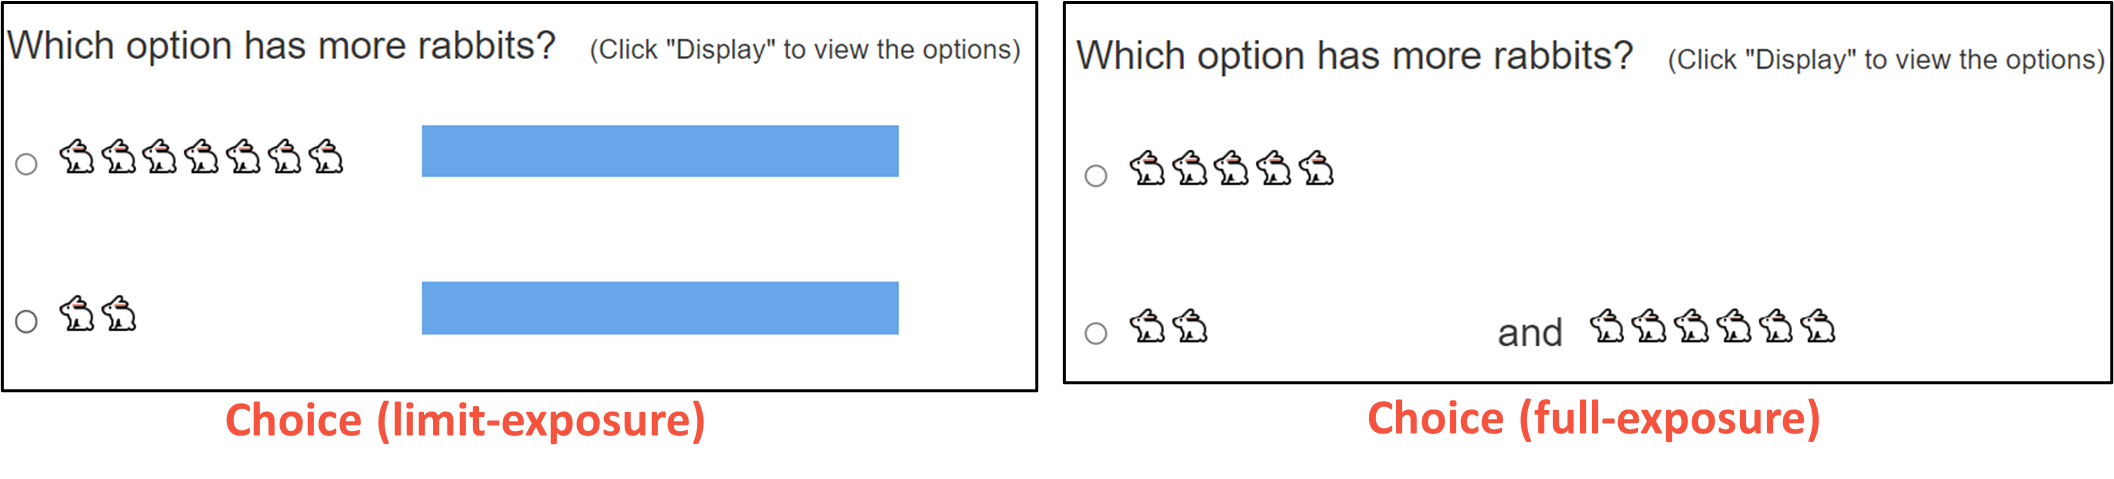
\includegraphics[width=\linewidth]{figures/exp3_screenshot_rabbit.png}
    \subcaption{Count-the-Rabbits Task}
  \end{subfigure}
  \caption{Example tasks in Experiment 1}
  \label{fig:exp3_screenshot}
\end{figure}

In each intertemporal choice task, the single option can be denoted by
``receive \(\eta\) today'' and the sequence option by ``receive
\(\rho \eta\) today and \(1.5(1-\rho)\eta\) in 12 months''. In other
words, by choosing the single option, a decision maker would get an
amount \((1-\rho)\eta\) more today than the front-end amount in the
sequence option; by choosing the sequence option, the same amount
\((1-\rho)\eta\) would be invested in a riskless bond and the decision
maker would get an interest of 50\% in one year later. Thus, the
preference for the sequence option is an indicator of patience. We
select \(\eta\) from \{£200, £240, £280, £320\} and \(\rho\) from \{0.1,
0.2, 0.3, 0.4, 0.5, 0.6\}. Overall, Part 1-2 contain 24 main tasks. We
randomly and evenly assign these tasks to each part. Except that, we add
an attention check task in each part and participants who fail one of
them will be excluded from the sample.\footnote{In one attention check
  task, each amount in the sequence option is £300 and the amount in the
  single option is £10. In the other attention check task, each amount
  in the sequence option is £80 and the amount in the single option is
  £300. Therefore, participants should definitely choose the sequence
  option in the former task and the single option in the latter task.}

In each count-the-rabbits task, suppose the single option contains
\(r_1\) rabbits, the first set of the sequence option contains \(r_2\)
rabbits, and the second set contains \(r_3\) rabbits. We select \(r_1\)
from \{7, 8\}, \(r_2\) from \{1, 2, 3\}. In half of these tasks, the
sequence option has one more rabbit than the single option
(\(r_2 + r_3 = r_1 + 1\)); for the other half, the single option has one
more rabbit than the sequence option (\(r_2 + r_3 = r_1 - 1\)). Overall,
there are 12 main tasks in Part 3-4. Similar to the intertemporal choice
tasks, we randomly and evenly assign these tasks to each part.

\hypertarget{altering-attention-through-goals}{%
\subsection{Altering Attention through
Goals}\label{altering-attention-through-goals}}

The difference between the two groups (limit-exposure/full-exposure)
lies in the information participants were exposed to when making
choices. Each participant experienced two parts (no question/question).
As is pointed out by \citet{chun2011taxonomy}, a critical function of
attention mechanisms is to ``focus limited processing capacity on the
most important information relevant to ongoing goals''. In the
``limit-exposure'' group, to achieve the goal of correctly answering the
additional questions, in each task participants have to remember the
(only) information being blocked out. Thus, in an intertemporal choice
task, during the forced viewing period they have to prioritize the
processing of the back-end amount in the sequence option, as this
information will never be accessible after that. By contrast, in the
``full-exposure'' group, all relevant information is visible when
participants answer the additional question, so they do not need to
specifically focus on that back-end amount.

Given the back-end amount is sizable, paying more attention to it should
make participants value the sequence option more. Therefore, for
intertemporal choice tasks, our hypothesis is that being required to
answer the additional question would increase participants' preference
for the sequence option within the ``limit-exposure'' group, and would
not have much impact on the choices of those within the
``full-exposure'' group.

The count-the-rabbits tasks help us understand the mechanisms by which
attention influences choices. As is pointed out by
\citet{pleskac2023attention}, attention can alter choices by two
possible processes: one is through valuation, the other is through
perception. The latter implies attention may increase the perceived
salience of an object and people intuitively tend to choose the more
salient option. In specific preferential and perceptual choice tasks,
\citet{pleskac2023attention} find evidence supporting the valuation
process and contradicting the perception process. For our experiment,
the count-the-rabbits tasks (perceptual choice) serve as an analog to
the intertemporal choice tasks (preferential choice). If attention
alters choice through perception, the groups and additional questions
should influence the choices in the same way for both kind of tasks.
Indeed, the results in Section \ref{exp3_intertemporal_result} and
Section \ref{exp3_rabbit_result} suggest they influence the choices in
each kind of tasks in different ways, thus supports the valuation
process.

\hypertarget{sample}{%
\subsection{Sample}\label{sample}}

We recruited 300 UK residents via Prolific (female: 152; mean age:
43.6). The median completion time is 10.1 minutes. Each participant was
paid £1.5 (on average £8.1 per hour). Four participants failed the
attention check. Besides, there were two participants for whom the tasks
were not displayed in the correct order.\footnote{For one of them, the
  data collected for main tasks in Part 2 ended up being the counterpart
  example tasks. For the other participant, the data collected for the
  example count-the-rabbit tasks in Part 3 ended up being intertemporal
  choice tasks.} We drop the participants who fail the attention check
and those for whom the tasks were not displayed correctly. In the end,
there are 148 participants in the ``full-exposure'' group and 146
participants in the ``limit-exposure'' group. We obtain 7,065
observations for intertemporal choice tasks and 3,504 observations for
count-the-rabbits tasks.

The accuracy rate for the additional questions in ``question'' parts is
high for each kind of tasks. For intertemporal choice tasks in Part 2,
the overall accuracy rate is 94.0\%, and 208 participants correctly
answered all questions. For count-the-rabbit tasks in Part 4, the
overall accuracy rate is 96.7\%, and 259 participants correctly answered
all questions.

\hypertarget{results}{%
\subsection{Results}\label{results}}

\hypertarget{intertemporal-choice-tasks}{%
\subsubsection{\texorpdfstring{Intertemporal Choice Tasks
\label{exp3_intertemporal_result}}{Intertemporal Choice Tasks }}\label{intertemporal-choice-tasks}}

Table \ref{tab:exp3_chi_test} illustrates how choices for the sequence
option vary across different kinds of tasks, groups and parts. For
intertemporal choice tasks, the proportion of choices for the sequence
option in the ``question'' part is 5.5\% higher than the ``no question''
part within the ``limit-exposure'' group, while within the
``full-exposure'' group, this difference is 2.1\%. For count-the-rabbits
tasks, the difference is 0.6\% within the ``limit-exposure'' group and
2.2\% within the ``full-exposure'' group. Results of \(\chi^2\)-tests
suggest the first difference, i.e.~the difference for intertemporal
choices in the ``limit-exposure'' group, is significant at the
significance level 0.1\% while the others are not significant.


\documentclass[12pt]{article}


\begin{document}
\begin{table}
    \caption{Comparing Choices Between Different Parts in Experiment 3}
    \vspace*{12pt}
    \centering

      \begin{tabular}{llllll}
\hline
 & Task & Group & \multicolumn{2}{r}{Part} & $chi^2$ \\
 &  &  & question & no question &  \\
\hline
 & Intertemporal Choice & limit-exposure & 0.523 & 0.468 & 10.303 ($p$=0.001) \\
 & Intertemporal Choice & full-exposure & 0.469 & 0.448 & 1.470 ($p$=0.225) \\
 & Count-the-Rabbits & limit-exposure & 0.463 & 0.474 & 0.147 ($p$=0.702) \\
 & Count-the-Rabbits & full-exposure & 0.515 & 0.476 & 2.470 ($p$=0.116) \\
\hline
\end{tabular}\hline

% INSERT chi_test_choice

    \vspace*{4pt}
    \centering
    \begin{minipage}{0.85\textwidth}
    {\par\footnotesize Note: For each kind of tasks and each group, the proportion of choices for the sequence option in each part (question/no question) is reported. In each row, we test whether the choices between the two parts follow the same distributions through $\Chi^2$-test. p-values are reported in parentheses. }
    \end{minipage}
    \label{tab:exp3_reg_response_time}
\end{table}

\end{document}



Further, we examine the impact of groups and questions on intertemporal
choices through a set of logistic linear regressions. Each regression
model is estimated through the maximum likelihood method. Table
\ref{tab:exp3_reg_intertemporal_choice} illustrates the key fixed-effect
estimates in the results. The dependent variable is 1 if a participant
choose the sequence option in a task and 0 otherwise. The variable Group
is 1 if the participant is in the ``limit-exposure'' group and 0
otherwise; Question is 1 if the task is within the ``question'' part and
0 otherwise. We construct a dummy variable for each individual task and
include these dummies as intercepts in regression models. For analysis,
we first assume the error is homoscedastic across the participants and
run a pooled regression on the full sample. Column (1) in Table
\ref{tab:exp3_reg_intertemporal_choice} show the results of this pooled
regression. Then, we add participant-specific dummies to the regression
model. In intertemporal choice tasks, there are some participants whose
choices are fixed at one option.\footnote{In the ``limit-exposure''
  group, 23 participants always choose the single-amount option and 21
  participants always choose the sequence option. In the
  ``full-exposure'' group, 31 participants always choose the
  single-amount option and 35 participants always choose the sequence
  option.} Including these participants in the regression with
participant-specific dummies will make the design matrix singular. We
apply two remedies to this. In Column (2), we run the regression on the
sample in which each participant has changed her choice at least once
across all intertemporal choice tasks. In Column (3), we run the
regression on the full sample, but represent the participants fixing at
one option with two only dummies: one for those always choose the
sequence option, and the other for those always choose the single
option.


\documentclass[12pt]{article}


\begin{document}
\begin{table}
    \caption{Regression Results for Intertemporal Choice Tasks}
    \vspace*{12pt}
    \centering

      \begin{tabular}{llll}
\hline
 & (1) Pooled & (2) FE & (3) FE \\
\hline
Group & 0.082 & 0.034 & -0.1 \\
 & (0.189) & (0.102) & (0.096) \\
Question$\cdot1\{\text{Group}=0\}$ & 0.084 & 0.289 & 0.289 \\
 & (0.059) & (0.185) & (0.183) \\
Question$\cdot1\{\text{Group}=1\}$ & 0.223$^{***}$ & 0.535$^{***}$ & 0.535$^{***}$ \\
 & (0.067) & (0.162) & (0.161) \\
$1\{\rho=0.2\}$ & -0.276$^{***}$ & -0.756$^{***}$ & -0.756$^{***}$ \\
 & (0.051) & (0.135) & (0.133) \\
$1\{\rho=0.3\}$ & -0.333$^{***}$ & -0.915$^{***}$ & -0.915$^{***}$ \\
 & (0.059) & (0.156) & (0.155) \\
$1\{\rho=0.4\}$ & -0.254$^{***}$ & -0.688$^{***}$ & -0.688$^{***}$ \\
 & (0.061) & (0.166) & (0.164) \\
$1\{\rho=0.5\}$ & -0.193$^{**}$ & -0.516$^{**}$ & -0.516$^{**}$ \\
 & (0.071) & (0.194) & (0.192) \\
$1\{\rho=0.6\}$ & -0.468$^{***}$ & -1.281$^{***}$ & -1.281$^{***}$ \\
 & (0.081) & (0.22) & (0.218) \\
$1\{s=240\}$ & 0.191$^{***}$ & 0.53$^{***}$ & 0.53$^{***}$ \\
 & (0.044) & (0.119) & (0.118) \\
$1\{s=280\}$ & 0.665$^{***}$ & 1.795$^{***}$ & 1.795$^{***}$ \\
 & (0.058) & (0.126) & (0.125) \\
$1\{s=320\}$ & 0.475$^{***}$ & 1.293$^{***}$ & 1.293$^{***}$ \\
 & (0.053) & (0.124) & (0.123) \\\hline

observations & 7056 & 4416 & 7056 \\
aic & 9621.97 & 4294.947 & 4303.619 \\
\hline
\end{tabular}
% INSERT reg_choice

    \vspace*{4pt}
    \centering
    \begin{minipage}{0.85\textwidth}
    {\par\footnotesize Note: * $p<0.05$, ** $p<0.01$, *** $p<0.001$. Standard errors are clustered at the subject level and are reported in the parentheses. The p-values are calculated based on Wald tests. FE denotes fixed effects. Subject-specific dummies are omitted in this table.}
    \end{minipage}
    \label{tab:manipulate_intertemporal_choice}
\end{table}

\end{document}



As is consistent with our hypothesis, in the ``limit-exposure'' group
(i.e.~Group = 1), participants are significantly more likely to choose
the sequence option within the ``question'' part than within the ``no
question'' part (For each column, \(p=0.001\)). By contrast, in the
``full-exposure'' group (i.e.~Group = 0), the additional questions do
not increase the preference for the sequence option by any significant
level.

\hypertarget{count-the-rabbits-tasks}{%
\subsubsection{\texorpdfstring{Count-the-Rabbits Tasks
\label{exp3_rabbit_result}}{Count-the-Rabbits Tasks }}\label{count-the-rabbits-tasks}}

In count-the-rabbits tasks, 226 participants correctly choose the option
with more rabbits for every task, and the overall accuracy rate is
97.0\%. There are only 105 wrong choices. As is illustrated in Figure
\ref{fig:exp3_wrong_rabbits}, the wrong choices in count-the-rabbits
tasks are disproportionally biased to the single option. In all
conditions except when participants do the ``question'' part within the
``full-exposure'' group, they are more likely to choose the single
option by mistake. A possible explanation for this is, in the
``full-exposure'' group, to answer the additional questions,
participants need to (and they can) count the rabbits within each bunch,
which helps eliminating the choice mistake.

\begin{figure}
  \centering
  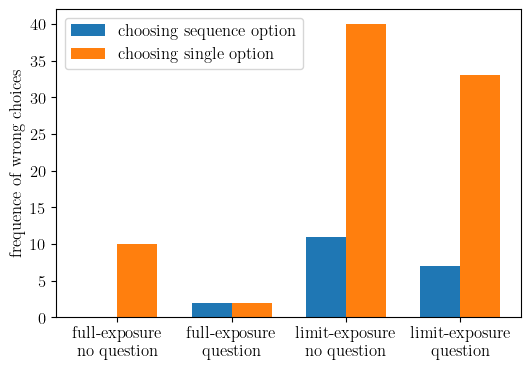
\includegraphics[width=0.7\linewidth]{figures/exp3_wrong_rabbit_choice.png}
  \caption{Frequence of wrong choices in count-the-rabbits tasks}
  \label{fig:exp3_wrong_rabbits}
\end{figure}

We conduct a set of logistic linear regressions upon the choices in the
count-the-rabbits tasks. Table \ref{tab:exp3_reg_rabbit_choice}
illustrates the key fixed-effect estimates. The dependent variable, and
the variable Group as well as Question are the same as for the
intertemporal choice tasks. Each task is treated as a dummy variable and
set as an intercept. Column (1) in Table
\ref{tab:exp3_reg_rabbit_choice} reports the results of a pooled
regression, while Column (2)-(4) report the results of a model with
participant-specific dummies. Column (2) is estimated on the full
sample, Column (3) is estimated on the sample in which each participant
has changed her choice at least once in intertemporal choice tasks,
Column (4) is estimated on the sample in which each participant has made
at least one wrong choice in count-the-rabbits tasks. Each column is
estimated through the maximum likelihood method.

The impact of additional questions on participants' choices, in
count-the-rabbits tasks, exihibits an opposite pattern to the
intertemporal choice tasks within each group. For count-the-rabbits
tasks, within the ``limit-exposure'' group, the additional questions
have no significant effect on choices; within the ``full-exposure''
group, the additional questions increase the increase the likelihood of
the sequence option being selected by a significant level (for Column
(1)-(4), the \(p\)-values are 0.011, 0.025, 0.017 and 0.009
respectively). By contrast, in intertemporal choice tasks, the
additional questions significantly increase the preference for the
sequence option for the ``limit-exposure'' group but not for the
``full-exposure'' group.


\documentclass[12pt]{article}


\begin{document}
\begin{table}
    \caption{Regression Results for Count-the-Rabbits Tasks}
    \vspace*{12pt}
    \centering

      \begin{tabular}{lllll}
\hline
 & (1) Pooled & (2) FE & (3) FE & (4) FE \\
\hline
Group & -0.73$^{*}$ & -4.379$^{***}$ & -0.158 & -0.757 \\
 & (0.33) & (1.114) & (8.618) & (0.392) \\
Question$\cdot1\{\text{Group}=0\}$ & 0.574$^{*}$ & 1.378$^{*}$ & 1.56$^{*}$ & 2.005$^{**}$ \\
 & (0.226) & (0.6) & (0.689) & (0.744) \\
Questsion$\cdot1\{\text{Group}=1\}$ & 0.062 & 0.152 & 0.391 & 0.145 \\
 & (0.318) & (0.368) & (0.422) & (0.344) \\
$1\{r_2 + r_3 > r_1\}$ & 7.797$^{***}$ & 11.71$^{***}$ & 11.198$^{***}$ & 6.181$^{***}$ \\
 & (0.377) & (1.091) & (1.249) & (0.552) \\
$1\{r_2 =2\}$ & 0.106 & 0.183 & 0.161 & 0.217 \\
 & (0.274) & (0.378) & (0.45) & (0.393) \\
$1\{r_2=3\}$ & -0.655$^{***}$ & -0.95$^{**}$ & -1.014$^{*}$ & -0.991$^{***}$ \\
 & (0.228) & (0.338) & (0.395) & (0.35) \\
$1\{r_1=8\}$ & 0.145 & 0.192 & 0.145 & 0.191 \\
 & (0.166) & (0.241) & (0.272) & (0.252) \\\hline

observations & 3504 & 3504 & 2190 & 810 \\
aic & 878.752 & 1100.636 & 746.754 & 583.857 \\
\hline
\end{tabular}
% INSERT reg_rabbit

    \vspace*{4pt}
    \centering
    \begin{minipage}{0.85\textwidth}
    {\par\footnotesize Note: * $p<0.05$, ** $p<0.01$, *** $p<0.005$. Standard errors are clustered at the subject level and are reported in the parentheses. The p-values are calculated based on Wald tests. FE denotes individual fixed-effects. Model (1)-(2) are run upon the full sample, (3) is for those having changed choices at least once in intertemporal choice tasks, (4) is for those having made wrong choices in count-the-rabbits tasks. Intercepts and subject-specific dummies are omitted in this table.}
    \end{minipage}
    \label{tab:exp3_reg_rabbit_choice}
\end{table}

\end{document}



\hypertarget{decision-times}{%
\subsubsection{Decision Times}\label{decision-times}}

To examine the participants' decision processes, we record the
participants' mouse position at the moment when they are prompted to
make a choice, i.e.~at the end of the forced viewing period, and their
response time in each choice task. The mouse position data suggest that
participants may form their intention to choose an option during the
forced viewing period, and the response times suggest blocking out
information in the sequence option may facilitate their choice for the
that option (though according to
\ref{tab:exp3_reg_intertemporal_choice}, this has no impact on their
time preferences).

First, the mouse position data indicate, during the forced viewing
period in each task, many participants tend to move their mouses toward
the option they eventually choose, though the mouse pointer is invisible
at that period.\footnote{Studies have suggested there is a strong
  relationship between the direction of mouse movements and subsequent
  decisions. For evidence, see \citet{freeman2010mousetracker} and
  \citet{freeman2018doing}.} Note the single option is presented above
the sequence option. As is illustrated in Figure
\ref{fig:exp3_screenshot}, when a participant click the ``Display''
button to view the content of options, her mouse pointer should lie in
the middle between the two options. After that, she can move mouse
freely until being asked to make a choice. In intertemporal choice
tasks, the average distance from the top of the screen to the mouse
pointer is 218px for those choosing the single option (on the top) but
264px for those choosing the sequence option (on the bottom). In
count-the-rabbit tasks, this average distance is 214px for those
choosing the single option and 248px for those choosing the sequence
option. Mann-Whitney \(U\) tests suggest, in each kind of tasks, the
vertical positions of mouse pointer for those choosing the single option
are significantly higher than those choosing the sequence option (for
intertemporal choice tasks, \(U = 9397658.5\), \(p<0.0001\); for
count-the-rabbits tasks, \(U=2122489.0\), \(p<0.0001\)). In Appendix, we
show in Figure \ref{fig:exp3_mouse_position} that, at the end of the
forced viewing period, the vertical positions of mouse pointer are
clustered exactly at the position of the option being chosen
subsequently. Therefore, we can infer that many participants are
developing their choices before some information is being block out, and
if our experimental conditions has a causal effect on choices, it is
highly likely that it occurs in the forced viewing period.

Second, we analyze the response times.\footnote{There are outliers in
  the response time data. For example, the longest time that a
  participant spent in an intertemporal choice is 349.39s while the
  average response time is 3.64s. To reduce the impact of outliers on
  our analysis, we remove the highest 0.5\% response times.} For
intertemporal choice tasks, the average response time is 3.41s for
choosing the single option and 3.62s for choosing the sequence option.
For count-the-rabbits tasks, the average response times are 3.80s and
4.88s respectively. Mann-Whitney \(U\) tests suggest response times for
choosing the single option are significantly shorter than for choosing
the sequence option (for intertemporal choice tasks, \(U = 2528314.5\),
\(p<0.003\); for count-the-rabbits tasks, \(U=739393.5\), \(p<0.0001\)).
Furthermore, we analyze the relationship between response times (in
second) and choices as well as experimental conditions through linear
regressions. The results suggest choices for the single option take
significantly less time, at the significance level 0.5\%. Table
\ref{tab:exp3_reg_response_time} of the Appendix provide more details of
these regressions. Therefore, choosing the single option might be more
intuitive in our tasks. This also explains why participants tend to
choose the single option by mistake in count-the-rabbits tasks.

\hypertarget{experiment-2-indifference-point}{%
\section{Experiment 2: Indifference
Point}\label{experiment-2-indifference-point}}

\hypertarget{design-1}{%
\subsection{Design}\label{design-1}}

In Experiment 2, we examine the impact of inattention to time attribute
and to small values on valuation of a reward sequence. We designed a
survey of 19 questions: it contains 14 fill-in-the-blank questions as
the main task, 4 choice questions for consistency check, and one
additional choice question measuring participants' impatience. For the
question measuring impatience, we use the ``Preference for Earlier vs
Later Income'' (PELI) task in \citet{burro2022patience}. The survey
begins with the consistency check questions, continues with the
fill-in-the-blank questions, and ends with the PELI question. At each
time, there is only one question on the screen. The questions are
developed with HTML and Javascript. We use JATOS \citep{lange2015just}
to deploy the survey.

Each fill-in-the-blank question in the main task contains two options -
Option A and Option B - framed as reward sequences. Option A offers two
positive rewards at two specific times: one is delivered today and the
other is delivered after a certain delay (e.g.~``receive £185 today and
£60 in 6 months''). Option B offers an unknown amount today and zero
amount after the same delay. Participants have to identify which level
of this unknown amount would make them value the two options equally,
and fill in their answer in a box. Figure \ref{fig:exp2_screenshot}
presents an fill-in-the-blank question in the main task. Before
participants start the main task, there is an example question helping
them get familiarized with the question format. Throughout the survey,
the back-end amount in Option A is fixed at £60. We set up two levels
for the sequence length (6 months, 12 months), and seven levels for the
front-end amount in Option A (£25, £105, £185, £265, £345, £425, £505) .
Overall, there are 14 fill-in-the-blank questions, presented in a random
order.

\begin{figure}   
  \vspace{16pt}   
  \centering   
  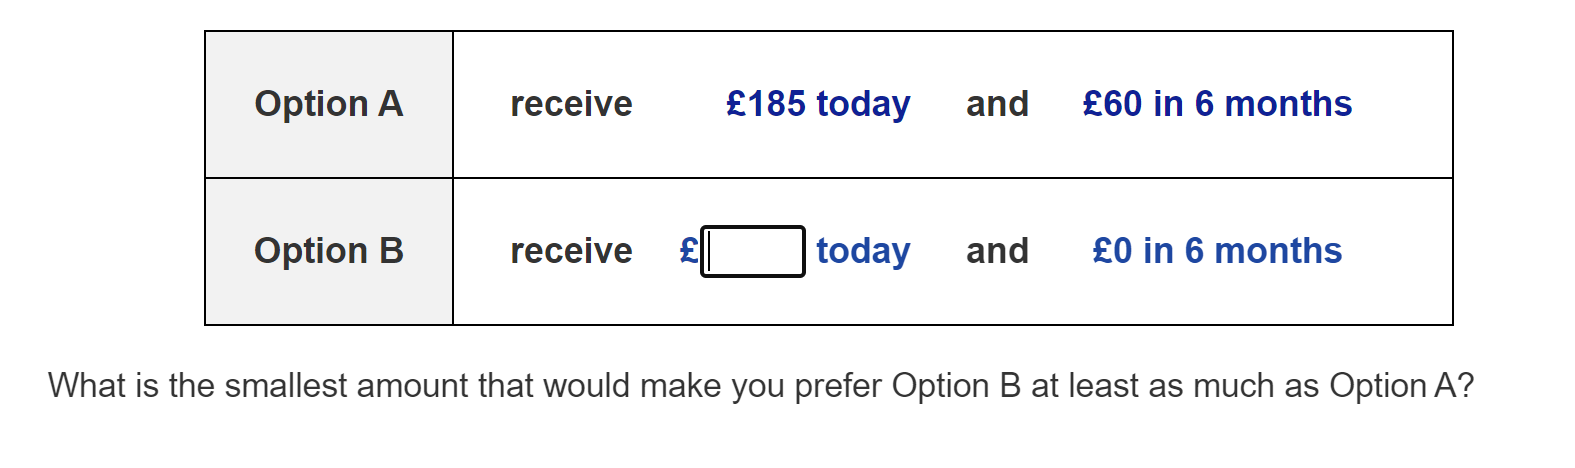
\includegraphics[width=0.96\textwidth]{figures/exp2_screenshot.png}    
  \caption{An fill-in-the-blank question in Experiment 2}   
  \label{fig:exp2_screenshot} 
\end{figure}

Each consistency check question also contains two options: one is the
same as the Option A of a subsequent fill-in-the-blank question, and the
other offers a specific amount today and zero amount in the future. The
amount offered today in the latter option, is either the same as the
back-end amount of the former option, or above the total money of the
former option. Participants are required to choose the option they
prefer. We exclude the participants whose choices are inconsistent with
their answers in the corresponding fill-in-the-blank questions. For
example, a participant may face a choice between ``receive £185 today
and £60 in 6 months'' and ``receive £300 today and £0 in 6 months''.
Suppose she chooses the latter, then it indicates she values the latter
option more, and for the corresponding fill-in-the-blank question, she
should fill in an amount smaller than £300.

\hypertarget{sample-1}{%
\subsection{Sample}\label{sample-1}}

We recruited 200 UK residents (female: 100; mean age: 40.5) via
Prolific. Three participants failed to complete the survey. For those
who completed the full survey, the median completion time is 5 minutes.
We pay each participant £1.2 (on average £14.26 per hour). There were
161 participants passing the consistency check. We remain the
participants passing the consistency check in our sample. Given that
each of them completed 14 fill-in-the-blank questions, we construct a
sample of 2,254 observations.

\hypertarget{results-1}{%
\subsection{Results}\label{results-1}}

\hypertarget{heterogeneity-in-decision-making}{%
\subsubsection{Heterogeneity in
Decision-Making}\label{heterogeneity-in-decision-making}}

In each question, Option A can be denoted by ``receive \(X_1\) today and
\(X_T\) in delay \(T\)'' and Option B can be denoted by ``receive \(Y\)
today and £0 in delay \(T\)''. The amount \(Y\) is filled by
participants and we call it the indifferent point between two options.
Taking receiving \(X_1\) now as the benchmark, by choosing the sequence
option people can receive an additional amount of \(X_T\) in delay
\(T\), and by choosing the single option they can receive an additional
amount of \(Y - X_1\) now. Thus, the present value of \(X_T\) is
revealed by \(Y-X_1\). For a certain \(X_T\), a smaller \(Y-X_1\)
indicates that people may discount the value of \(X_T\) more.

Figure \ref{fig:exp2_response_dist}(a) illustrates the distribution of
indifference points for each question. Note in Option A, the back-end
amount is fixed at £60. The y-axis of this subfigure is the indifference
point minus front-end amount, i.e.~\(Y-X_1\). 86.4\% of the observations
lie in the range from £0 to £60; 12.8\% of the observations are above
£60, implying that some participants value Option A as much as receiving
an amount greater than its total money today; 0.8\% of the observations
is negative, implying that some the participants value Option A as much
as receiving an amount lower than its front-end amount today. The latter
two could originate from various causes, e.g.~the discount factor
\(w_T\) is too large,\footnote{Suppose in Equation (1), \(w_T\) is close
  to 1, then the decision maker needs a \(u(Y)\) almost equal to
  \(u(X_1)+u(X_T)\). Given \(u(.)\) is strictly concave, it is not
  impossible that \(Y>X_1+X_T\).} participants made mistakes or
over-rounded when filling in answers. Some observations in the latter
two cases should be viewed as outliers. For example, the maximum and
minimum levels of \(Y-X_1\) are £375 and -£265.\footnote{For the maximum
  case, the participant values ``receive £425 today and £60 in 12
  months'' as much as receiving £800 today, but values ``receive £505
  today and £60 in 6 months'' as much as receiving £505 today. For the
  minimum case, the participant values ``receive £425 today and £60 in
  12 months'' as much as receiving £160 today, but for all the other
  questions, the \(Y-X_1\) is ranged between £15 and £60. Thus, it is
  likely that such observations are mistakes.}

In addition, a substantial proportion of indifference points (43.8\%)
are simply \(X_1 + X_T\), i.e.~the total money to be obtained in Option
A. Such ``\emph{total money}'' answers are highly likely to be a
heuristic because on average these answers take less time (9.28s) than
the other answers (10.88s), and the difference is significant
(two-sample test: \(t=4.177\), \(p<0.0001\)). Figure
\ref{fig:exp2_response_dist}(b) illustrates the distribution of ``total
money'' answers over the participants. There are two peaks in the
distribution: of all 161 participants in our sample, 62 participants
(38.5\% of the participants) use the total money to answer every
question, whereas 65 participants have never used the total money as an
answer. This suggests, different people may use different approaches to
value the sequence Option A, and the ``total money'' is one of those
approaches. For those who consistently fill in the total money across
the questions, their valuation of the sequence Option A cannot be
explained by time discounting. As we illustrate above, we account for
this behavior by inattention to the time attribute.

\begin{figure}
    \centering
    \begin{subfigure}{0.5\textwidth}
        \centering
        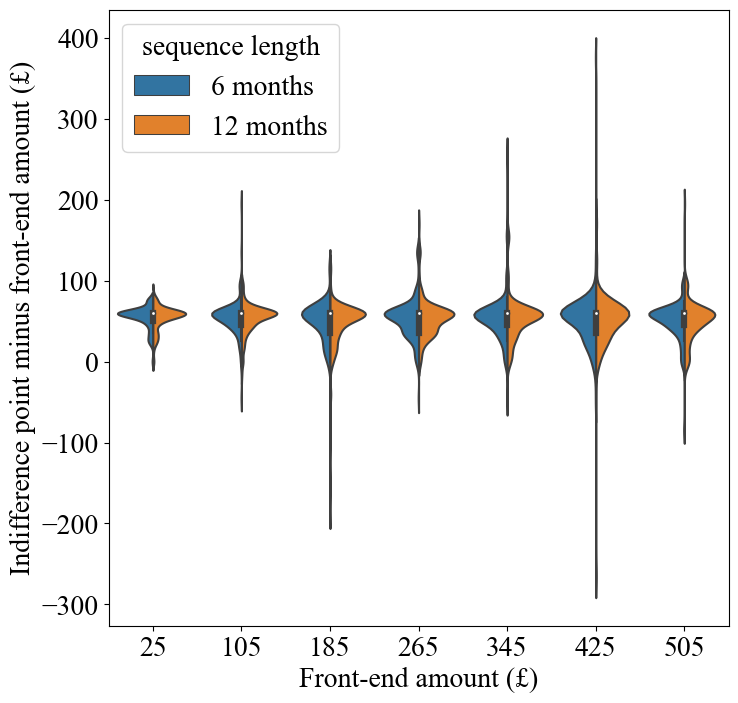
\includegraphics[width=\linewidth]{figures/exp2_dist_indiff_point.png} 
        \subcaption{}
    \end{subfigure}
    \hfill
    \begin{subfigure}{0.49\textwidth}
        \centering
        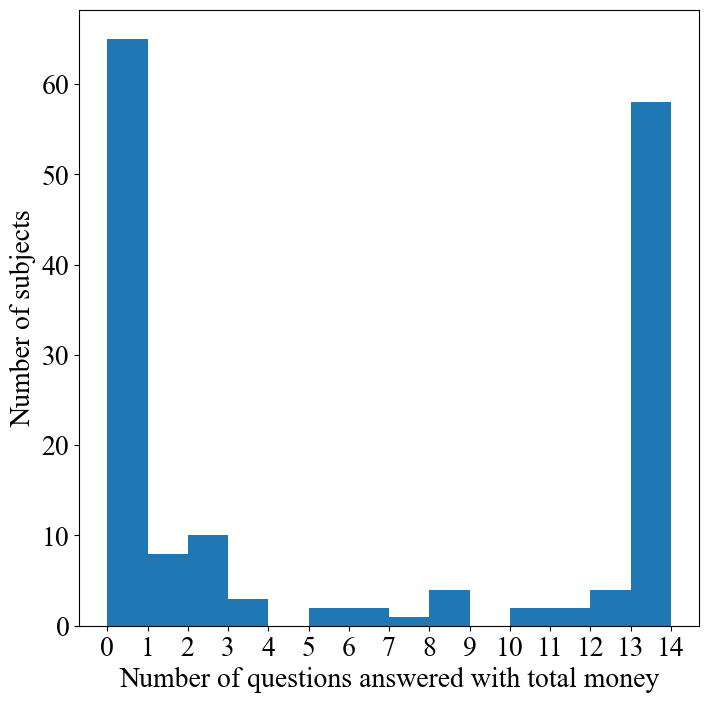
\includegraphics[width=\linewidth]{figures/exp2_dist_sum_heuristic.png}
        \subcaption{}
    \end{subfigure}
    \caption{Distribution of responses in Experiment 2}
    \label{fig:exp2_response_dist}
\end{figure}

We then use the k-means method to cluster participants into two groups,
based on their answers in all questions. The first group (cluster 1) has
104 participants, and the second (cluster 2) has 57
participants.\footnote{In the case that there are three clusters, the
  number of participants in each cluster is 105, 55 and 1. In the case
  of four clusters, the number of participants in each cluster is 105,
  46, 1 and 9. We only divide people into two groups because the size
  for the third (and fourth) group is too small.} The Mann-Whitney \(U\)
test rejects the hypothesis that the two clusters are drawn from a same
population (\(U=1059304.0\), \(p<0.0001\)). The proportion of the
``total money'' answers is 63.1\% in cluster 1, and is only 8.6\% in
cluster 2, and the difference is significant (Pearson's
\(\chi^2 = 619.040\), \(p<0.0001\)). Over 79\% of the observations in
cluster 2 are above £0 and lower than £60. Thus, people in cluster 1 are
disporportionally more likely to use total money to value a reward
sequence, while those in cluster 2 are more likely to value it through
time discounting approach.

Figure \ref{fig:exp2_cluster} shows the median and mean indifference
point minus the back-end amount £60, for each question. The patterns of
lines also suggest that people in cluster 1 tend to use the total money
in answers, and for people in cluster 2, \(Y - X_1\) is decreasing with
\(X_1\). The former is better explained by inattention to time attribute
rather than by time discounting, as we discuss in Section
\ref{attention_time}. The latter violates the popular assumption that
time discounting is solely dependent on times, as we discuss in Section
\ref{impli_indiff_point}.

\begin{figure}
    \centering
    \begin{subfigure}{0.51\textwidth}
        \centering
        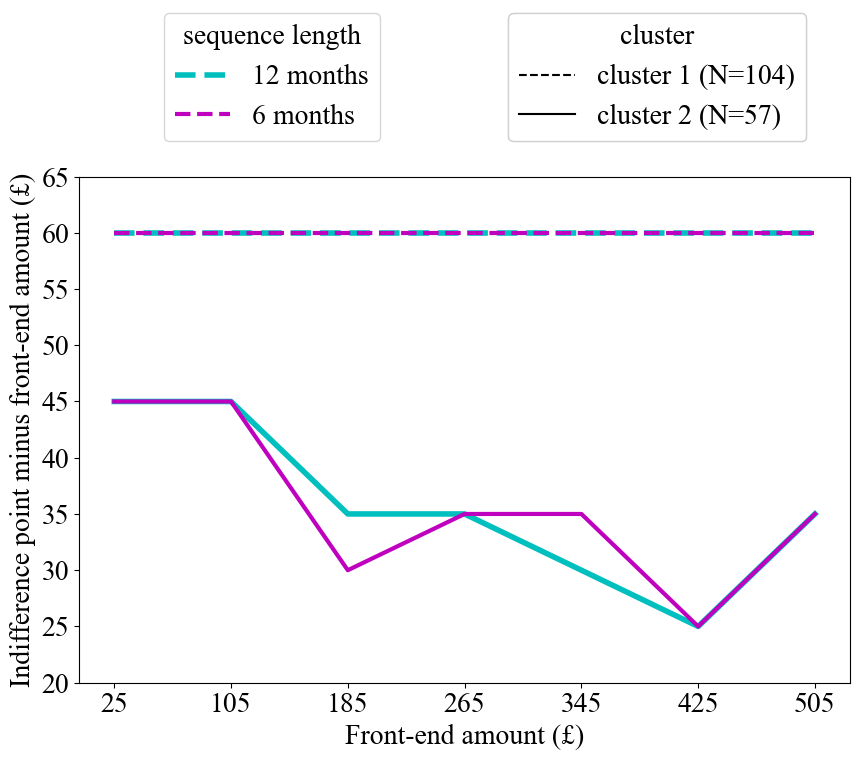
\includegraphics[width=\linewidth]{figures/exp2_cluster_result_median.png} 
        \caption{median}
    \end{subfigure}
    \hfill
    \begin{subfigure}{0.48\textwidth}
        \centering
        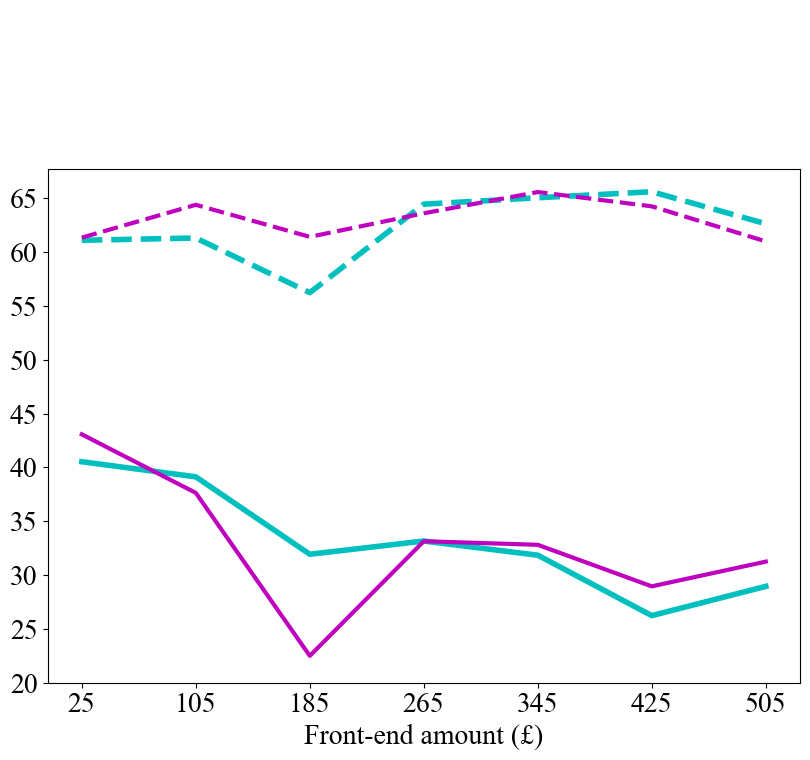
\includegraphics[width=\linewidth]{figures/exp2_cluster_result_mean.png}
        \caption{mean}
    \end{subfigure}
    \caption{Median and mean indifference point minus the front-end amount for each fill-in-the-blank question}
    \label{fig:exp2_cluster}
\end{figure}

\hypertarget{large-front-end-amount-devalues-the-back-end-amount}{%
\subsubsection{Large Front-End Amount Devalues the Back-End
Amount}\label{large-front-end-amount-devalues-the-back-end-amount}}

We analyze the relationship between \(Y - X_1\) and \(X_1\) while taking
into account the heterogeneity in participants' decision processes. The
key question is, for people answer the questions in a way apart from
``total money'', whether \(Y-X_1\) is decreasing in \(X_1\). Notably,
the sample contains outliers which may influence our results. We deal
with the outliers in three ways. First, we use nonparametric methods for
a preliminary analysis. Second, we validate the findings in linear
regressions. The regression models are estimated through the OLS method.
To reduce the impact of outliers, we remove the most extreme 0.5\% of
observations (the six largest and six smallest \(Y-X_1\)) from the
sample. Third, we conduct robust regressions using Huber's M-estimators
on the full sample, as such estimators are generally insensitive to
outliers \citep{huber2009robust}.

We first look at the nonparametric analysis. The Spearman's \(\rho\)
between \(Y - X_1\) and \(X_1\) is -0.049, which indicates a weak
negative correlation between them (\(p=0.021\)). For people in cluster
1, the Spearman's \(\rho\) is -0.015 (\(p=0.556\)); for people in
cluster 2, the Spearman's \(\rho\) is -0.189 (\(p<0.0001\)). This
indicates \(Y-X_1\) is irrelevant to \(X_1\) in cluster 1, but
significantly decreasing in \(X_1\) in cluster 2. Furthermore, the
results from Kendall's \(\tau\) coefficient is similar. For all
participants, the Kendall's \(\tau\) between \(Y-X_1\) and \(X_1\) is
-0.038 (\(p=0.018\)). For people in cluster 1, the Kendall's \(\tau\) is
-0.013 (\(p=0.552\)); for people in cluster 2, the Kendall's \(\tau\) is
-0.148 (\(p<0.0001\)).

Then we run a set of linear regressions to predict \(Y- X_1\). The
independent variables are the front-end amount \(X_1\) under each
sequence length \(T\), and participants' responses to the PELI question.
The variable PELI is 1 if a participant chooses the large later income
in the PELI question and 0 if she chooses the small earlier income.
Meanwhile, we use variables CL1 and CL2 to represent clustering results,
and construct interaction terms between them and \(X_1\) under each
sequence length \(T\). The variable CL1 is 1 if a participant is in
cluster 1 and 0 otherwise; CL2 is 1 if a participant is in cluster 2 and
0 otherwise.


\documentclass[12pt]{article}


\begin{document}
\begin{table}
    \caption{Regression results for Experiment 2}
    \vspace*{12pt}
    \centering

      \begin{tabular}{lllllll}
\hline
& (1) Pool & (2) Pool & (3) FE & (4) FE & (5) RLM & (6) RLM \\
\hline
$X_1\cdot1\{T=T_L\}$ & -0.006$^{***}$ &  & -0.006$^{**}$ &  & -0.005$^{***}$ &  \\
 & (0.002) &  & (0.002) &  & (0.001) &  \\
$X_1\cdot1\{T=T_H\}$ & -0.006$^{***}$ &  & -0.006$^{**}$ &  & -0.007$^{***}$ &  \\
 & (0.002) &  & (0.002) &  & (0.001) &  \\
$X_1\cdot1\{T=T_L\}\times$CL1 &  & 0.023$^{***}$ &  & 0.002 &  & 0.0 \\
 &  & (0.004) &  & (0.002) &  & (0.001) \\
$X_1\cdot1\{T=T_H\}\times$CL1 &  & 0.024$^{***}$ &  & 0.003 &  & -0.0 \\
 &  & (0.004) &  & (0.002) &  & (0.001) \\
$X_1\cdot1\{T=T_L\}\times$CL2 &  & -0.06$^{***}$ &  & -0.02$^{***}$ &  & -0.018$^{***}$ \\
 &  & (0.005) &  & (0.004) &  & (0.002) \\
$X_1\cdot1\{T=T_H\}\times$CL2 &  & -0.061$^{***}$ &  & -0.022$^{***}$ &  & -0.022$^{***}$ \\
 &  & (0.005) &  & (0.004) &  & (0.002) \\
PELI & -0.705 & -1.218 & 8.796$^{***}$ & 6.52$^{***}$ & 1.431$^{***}$ & 1.439$^{***}$ \\
 & (3.815) & (2.552) & (0.014) & (0.392) & (0.33) & (0.322) \\
Constant & 54.194$^{***}$ & 54.586$^{***}$ & 46.971$^{***}$ & 48.711$^{***}$ & 52.766$^{***}$ & 53.026$^{***}$ \\
 & (3.461) & (2.603) & (0.507) & (0.449) & (0.375) & (0.365) \\\hline

observations & 2242 & 2242 & 2242 & 2242 & 2254 & 2254 \\
adj-$R^2$ & 0.001 & 0.335 & 0.637 & 0.645 &  &  \\
Muller-Welsh &  &  &  &  & 146.734 & 139.589 \\
\hline
\end{tabular}
% INSERT reg_combined

    \vspace*{4pt}
    \centering
    \begin{minipage}{1.0\textwidth}
    {\par\footnotesize Note: * $p<0.05$, ** $p<0.01$, *** $p<0.005$. Standard errors are reported in the parentheses. Column (1)-(2) are obtained from pooled OLS models, Column (3)-(4) are from fixed-effect OLS models, Column (5)-(6) are from fixed-effect robust linear models (RLM). For OLS, standard errors are clustered at the subject level, and p-values are calculated using t-tests. For RLM, each model is estimated using Huber's M-estimator (the threshold for loss function is set at 1.345) and the scale estimator is Huber's proposal 2 estimator. Each $p$-value for RLM is calculated based on a normal distribution with i.i.d. assumption. $Y_1$ and $T$ denote the front-end amount and the sequence length in Option A. $T_L$ and $T_H$ are 6 months and 12 months, respectively. Clustering results are obtained through the k-means method.}
    \end{minipage}
    \label{tab:exp2_seq_value_reg}
\end{table}

\end{document}



Table \ref{tab:exp2_seq_value_reg} illustrates the regression results.
Column (1)-(2) are the pooled OLS regressions run on the sample without
outliers. The adjusted \(R^2\) for the two columns indicates that
incorporating clustering results in regression models improves the
goodness of fit by a lot (from 0.001 to 0.335). Then we add
participant-specific dummies into each model and run fixed-effect
regressions. First, we estimate the models on the sample without
outliers, using the OLS method. Second, we estimate the same models on
the full sample, using Huber's M-estimator for loss function and Huber's
proposal 2 estimator for scale estimator. Column (3)-(4) report the
fixed-effect estimates obtained from the OLS regressions, and Column
(5)-(6) report the estimates obtained from the Huber's robust
regressions. Under each estimator, these fixed-effect models yield
similar results. Overall, \(Y-X_1\) is slightly decreasing with the
front-end amount \(X_1\). For participants in cluster 1, an increase in
\(X_1\) has no significant impact on how people value the back-end
amount. But for those in cluster 2, this increase significantly reduces
\(Y-X_1\), at the significance level 0.5\%. It is also worth noting
that, for people in cluster 2, according to Column (6), an £100 increase
in \(X_1\) reduces its revealed present value, \(Y-X_1\), by £1.8 when
the sequence is 6-month long, and by £2.2 when the sequence is 12-month
long, which are 3.0\% and 3.7\% of the amount £60.\footnote{For robust
  regressions, we use the Muller-Welsh criterion to measure the model
  performance \citep{muller2005outlier}. A smaller Mull-Welsh score
  implies a greater ability to parsimoniously fit the data and predict
  new independent observations. The calculation of the Muller-Welsh
  criterion requests applying stratified bootstrap. To construct
  bootstrap samples, we divide observations into three strata (the upper
  tail, the lower tail, the others), and draw observations with
  replacement within each stratum. Each bootstrap sample is 50\% in size
  of the entire sample, and the process is repeated 1,000 times. Column
  (6) has a better performance in this criterion.}

For Column (5)-(6), in case the residuals are not normally distributed
due to outliers, we obtain the confidence intervals of regression
coefficients via a stratified bootstrap method, In Appendix, Figure
\ref{fig:exp2_bootstrap_ci} illustrate the bootstrap 95\% confidence
intervals for key fixed-effect estimates. The results in Table
\ref{tab:exp2_seq_value_reg} remain robust to this bootstrap method.
Moreover, as a robustness check, we use the Gaussian mixture model,
instead of k-means, to cluster participants into two groups. The
Gaussian mixture model exactly groups the participants who answer every
question with the ``total money'' (N=62) into cluster 1, and the
remaining 99 participants into cluster 2. We run the same regressions
based on the new clustering results. In Appendix, Figure
\ref{fig:exp2_bootstrap_ci_gmm} illustrates the bootstrap 95\%
confidence intervals of the key fixed-effect estimates in a model
corresponding to Column (6). Our results remain robust under this
circumstance.

\hypertarget{correlation-between-valuation-approach-and-patience}{%
\subsubsection{Correlation between Valuation Approach and
Patience}\label{correlation-between-valuation-approach-and-patience}}

The coefficients for PELI in Table \ref{tab:exp2_seq_value_reg} are all
significantly positive at the significance level 0.5\%. This suggest
that people who choose the large later income rather than the small
earlier income in the PELI question tend to value the back-end amount at
a higher level. Thus, the PELI question provides a valid measure for
patience in our experiment. The Mann-Whitney \(U\) test on \(Y-X_1\)
also rejects the hypothesis that participants choosing different options
in the PELI question are drawn from the same population (\(U=421520.0\),
\(p=0.004\)).

The relationship between participants' choices in the PELI questions and
how they value the sequence Option A is ambiguous. Putting the k-means
clustering results and the variable PELI into a contingency table, we
obtain \(\chi^2 = 0.550\), \(p=0.458\), which indicates the clusters and
PELI are not correlated. However, using the Gaussian mixture model as
the clustering method lead to an opposite result. In the latter case,
\(\chi^2\)-test suggests those exhibiting more patience in the PELI
question, i.e.~choosing the large later income, are more likely to use
the total money answering all questions in the main task
(\(\chi^2 = 11.063\), \(p = 0.001\)).

\hypertarget{experiment-3-sensitivity-of-choice-probability}{%
\section{Experiment 3: Sensitivity of Choice
Probability}\label{experiment-3-sensitivity-of-choice-probability}}

\hypertarget{design-2}{%
\subsection{Design}\label{design-2}}

In Experiment 3, we further test how (in-)attention to small values may
affect time discounting. Specifically, we test Proposition 1 and
Proposition 2 with an online survey. The survey consists of 20
intertemporal choices questions and 3 risky choices questions. Each
question is presented as a choice list. In an intertemporal choice
question, there are 10 rows in the list. In each row, participants are
required to choose between a single immediate reward (``option A'') and
a sequence of two positive rewards (``option B''). Option A is constant
within a question, while option B varies from row to row. Participants
need to actively state their preferences on each choice. The
intertemporal choice questions are presented in a random order and two
of them are used for attention check. Figure \ref{fig:exp1_screenshot}
present an intertemporal choice question in the survey. Before the
survey begins, there is an example question helping participants get
familiarized with this question format. The risky choice questions
follow the same format. In each row of a risky choice question,
participants can choose to get either a large reward with a 50\% chance,
or a small reward with certainty. The risky reward is constant within
the question, while the safe reward varies across rows. We use these
risky choice questions to characterize the participants' utility
function for further analysis.\footnote{Each risky choice question has 7
  rows and the safe reward amount increases by the same amount with each
  row. The amount in the risky reward option (constant across rows) is
  selected from \{£50, £100, £180\}. For amount £50, the safe reward
  amount varies from £3 to £27; for amount £100, the safe reward amount
  varies from £20 to £50; for amount £180, the safe reward amount varies
  from £30 to £90.}

The intertemporal choice questions are divided into two conditions: (1)
\emph{front-end amount varies}; (2) \emph{back-end amount varies}. In
each question under the ``front-end amount varies'' condition, the
front-end amount in the sequence option increases by £10 with each row,
starting from £10 and going up to £100, whereas the back-end amount
remains constant for all rows. In each question under the ``back-end
amount varies'' condition, the back-end amount varies across rows,
following the same pattern as the first condition, while the front-end
amount remains constant. Under each condition, the time length of the
sequence option is also constant across rows in a choice list.

\begin{figure}   
  \vspace{16pt}   
  \centering   
  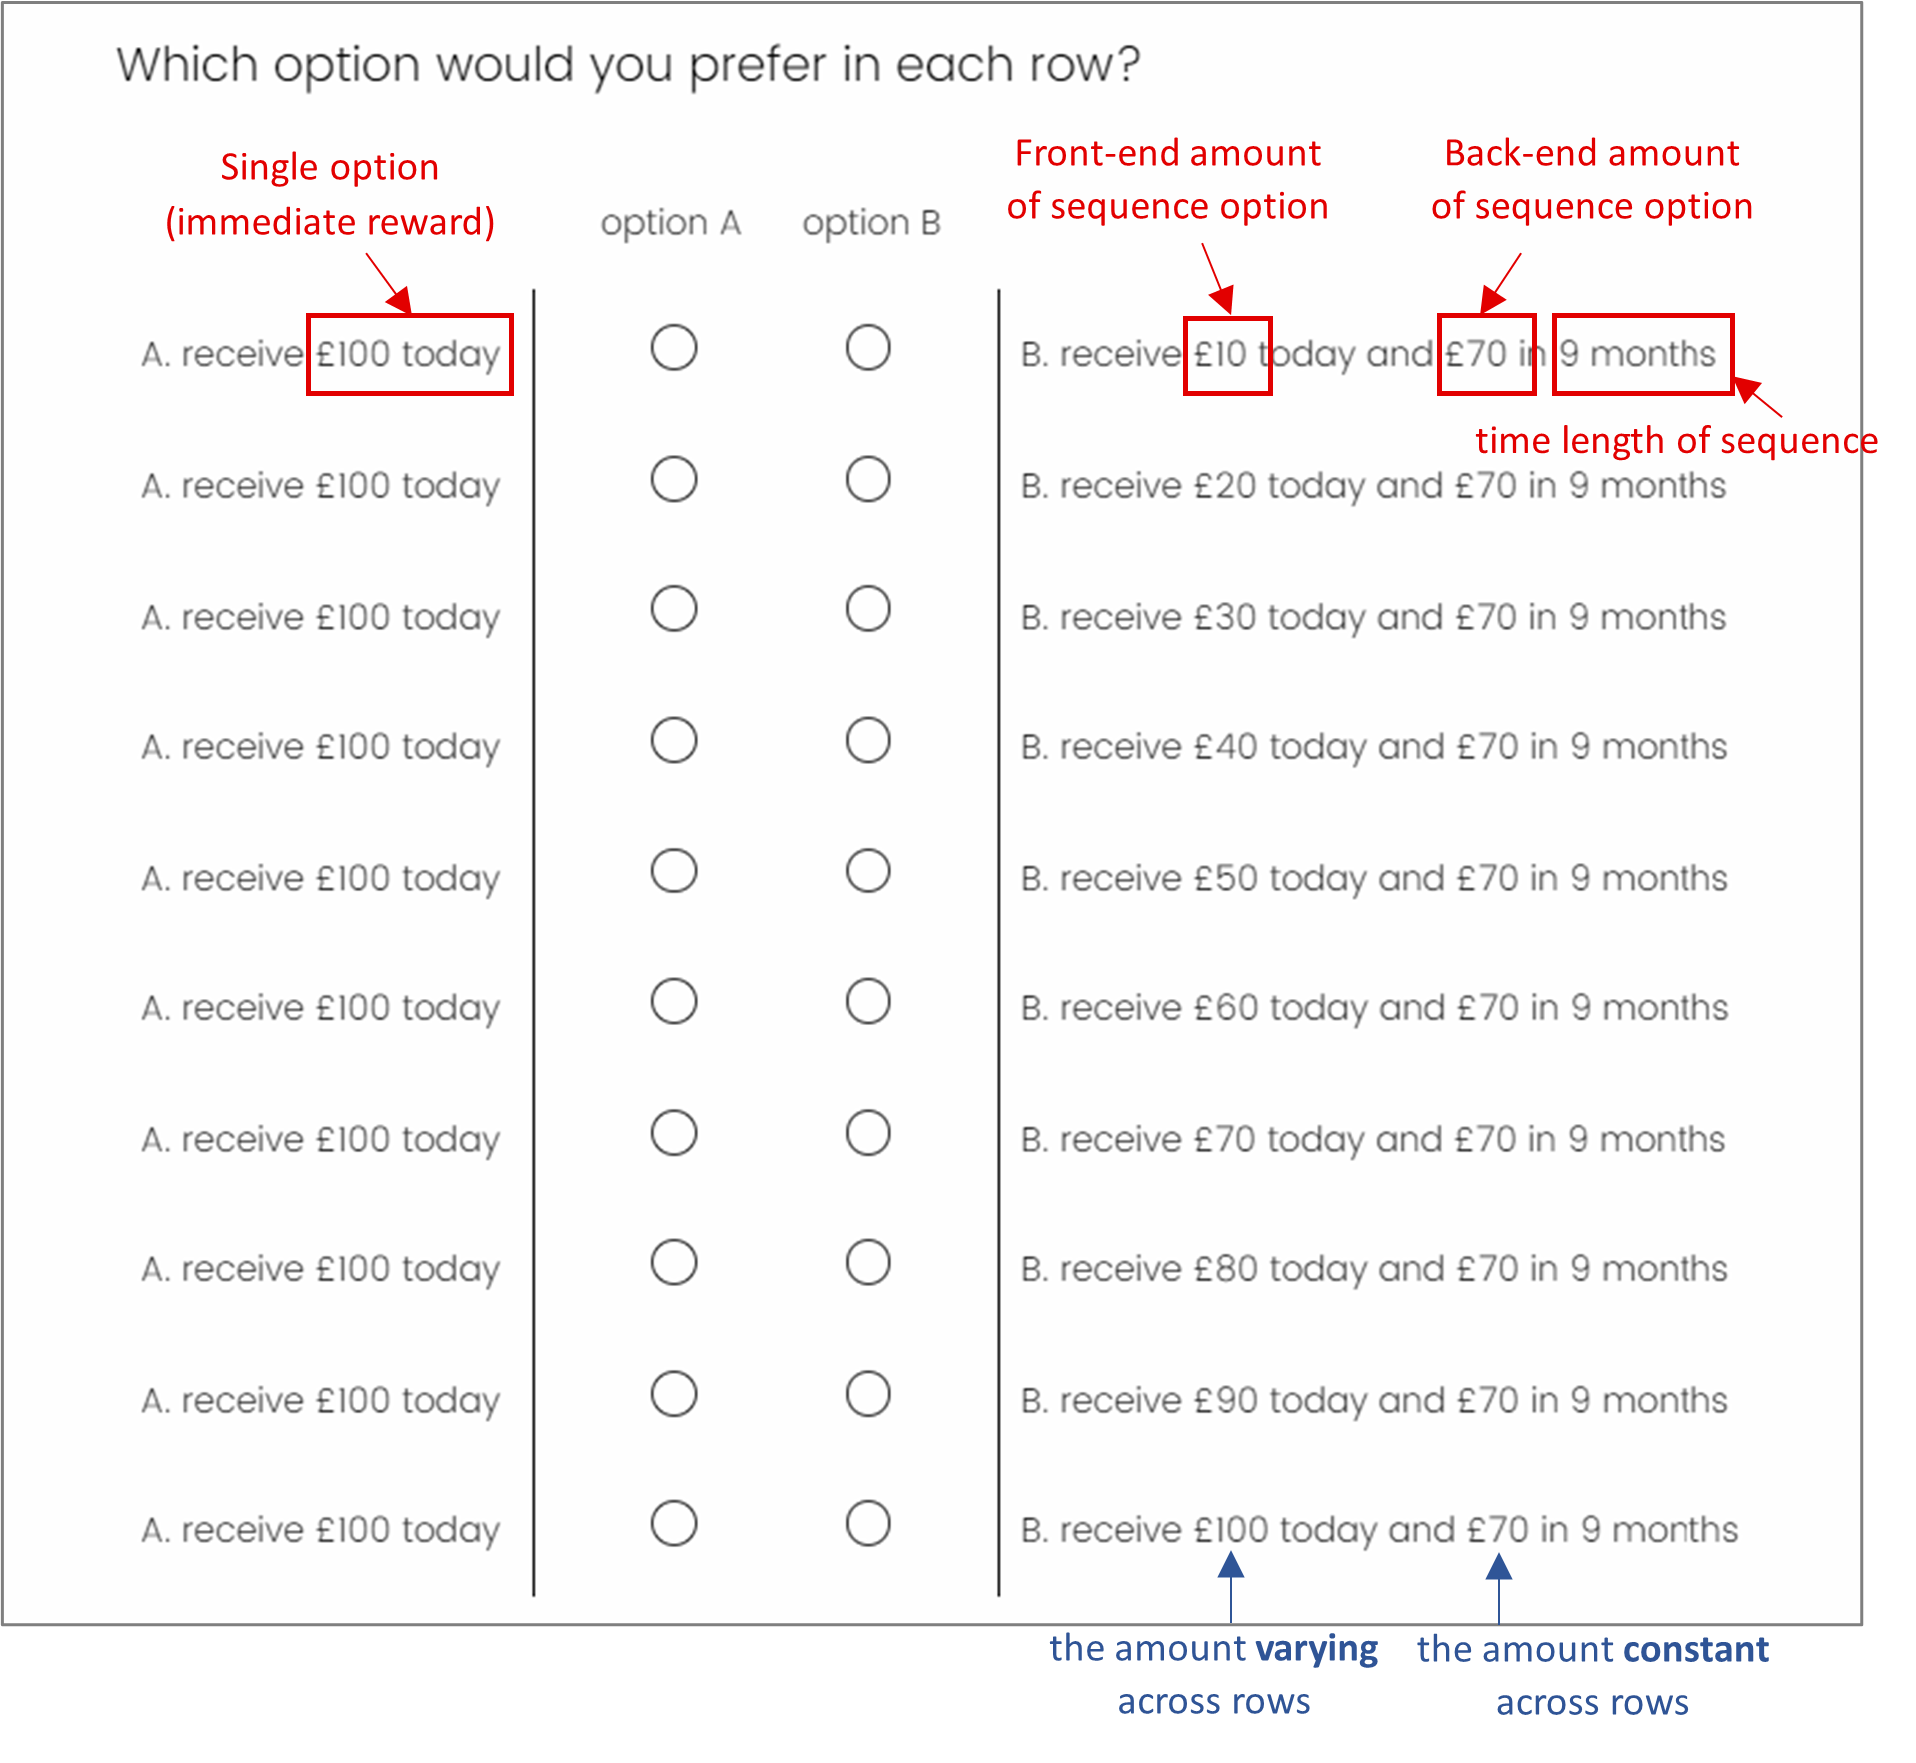
\includegraphics[width=0.96\textwidth]{figures/exp1_screenshot.png}   
  \caption{An intertemporal choice question in Experiment 1}  
  \label{fig:exp1_screenshot} 
\end{figure}

The amount of the single option is selected from \{£100, £120\}. Each of
such amounts is paired with a combination of a amount constant across
rows and a specific length of the sequence option. Under the ``front-end
amount varies'' condition, the length of a sequence is selected from \{1
month, 9 months, 18 months\}, and the back-end amount, which is constant
across rows, is selected from \{£50, £70, £90\}. The lowest level of the
back-end amount (£50) is only combined with the shortest sequence length
(1 month), the middle level of the back-end amount (£70) can be combined
with the shortest or middle level of sequence length (1 month or 9
months), and the highest level of the back-end amount can be combined
with any level of sequence length (1 month, 9 months or 18 months). By
this approach, we ensure that in any question, most people would switch
their preference in the middle of the choice list. Eventually, we obtain
6 combinations, and by pairing them with each amount of the single
option, we obtain 12 questions for the first condition. Under the
``back-end amount varies'' condition, we only examine whether the impact
of each unit change in the back-end amount on choices will be influenced
by the other amount in the sequence. So, the sequence length is simply
fixed at 3 months. Under this condition, the front-end amount, which is
constant across rows, is selected from \{£50, £70, £90\} as well.
Pairing them with each amount of the single option, we obtain 6
questions for the second condition. Overall, there are 18 intertemporal
choice questions except for attention check questions.

\hypertarget{sample-2}{%
\subsection{Sample}\label{sample-2}}

We recruited 160 UK residents (female: 80, mean age: 41.9) via Prolific.
The survey is developed and deployed with Qualtrics. The median survey
completion time is 10 minutes. Each participants received £2 after
completing the survey (on average £11.94 per hour). Three participants
failed the attention check and we remove them from the sample.
Eventually, there are 157 participants in the sample. Each participants
completed 12 intertemporal choice questions under the ``front-back
amount varies'' condition and 6 questions under the ``back-end amount
varies'' condition. Each row in an intertemporal choice question is
taken as an observation. Given that each intertemporal choice question
contains 10 rows, we obtain 18,840 observations for the first condition
and 9,420 observations for the second condition. For risky choice
questions, we obtain 3,297 observations.

\hypertarget{results-2}{%
\subsection{Results}\label{results-2}}

\hypertarget{sensitivity-to-front-end-amount-is-modulated-by-back-end-amount}{%
\subsubsection{Sensitivity to Front-End Amount Is Modulated by Back-End
Amount}\label{sensitivity-to-front-end-amount-is-modulated-by-back-end-amount}}

We start by presenting the results of descriptive analysis and then move
on to regression analysis. For every choice list, we identify each
participant's indifference point between the left and right sides by the
median of the rows where she switches from choosing the single option to
the sequence option. If the participants choose the single (sequence)
option for every row in the choice list, we set the indifference point
as the maximum (minimum) row. Note the single option and one amount in
the sequence option are fixed in a choice list, hereafter we refer to
the indifference point with the only amount varying across rows. Figure
\ref{fig:exp1_indiff_sd} shows the standard deviation of such
indifference points for each question.

\begin{figure}   
  \centering   
  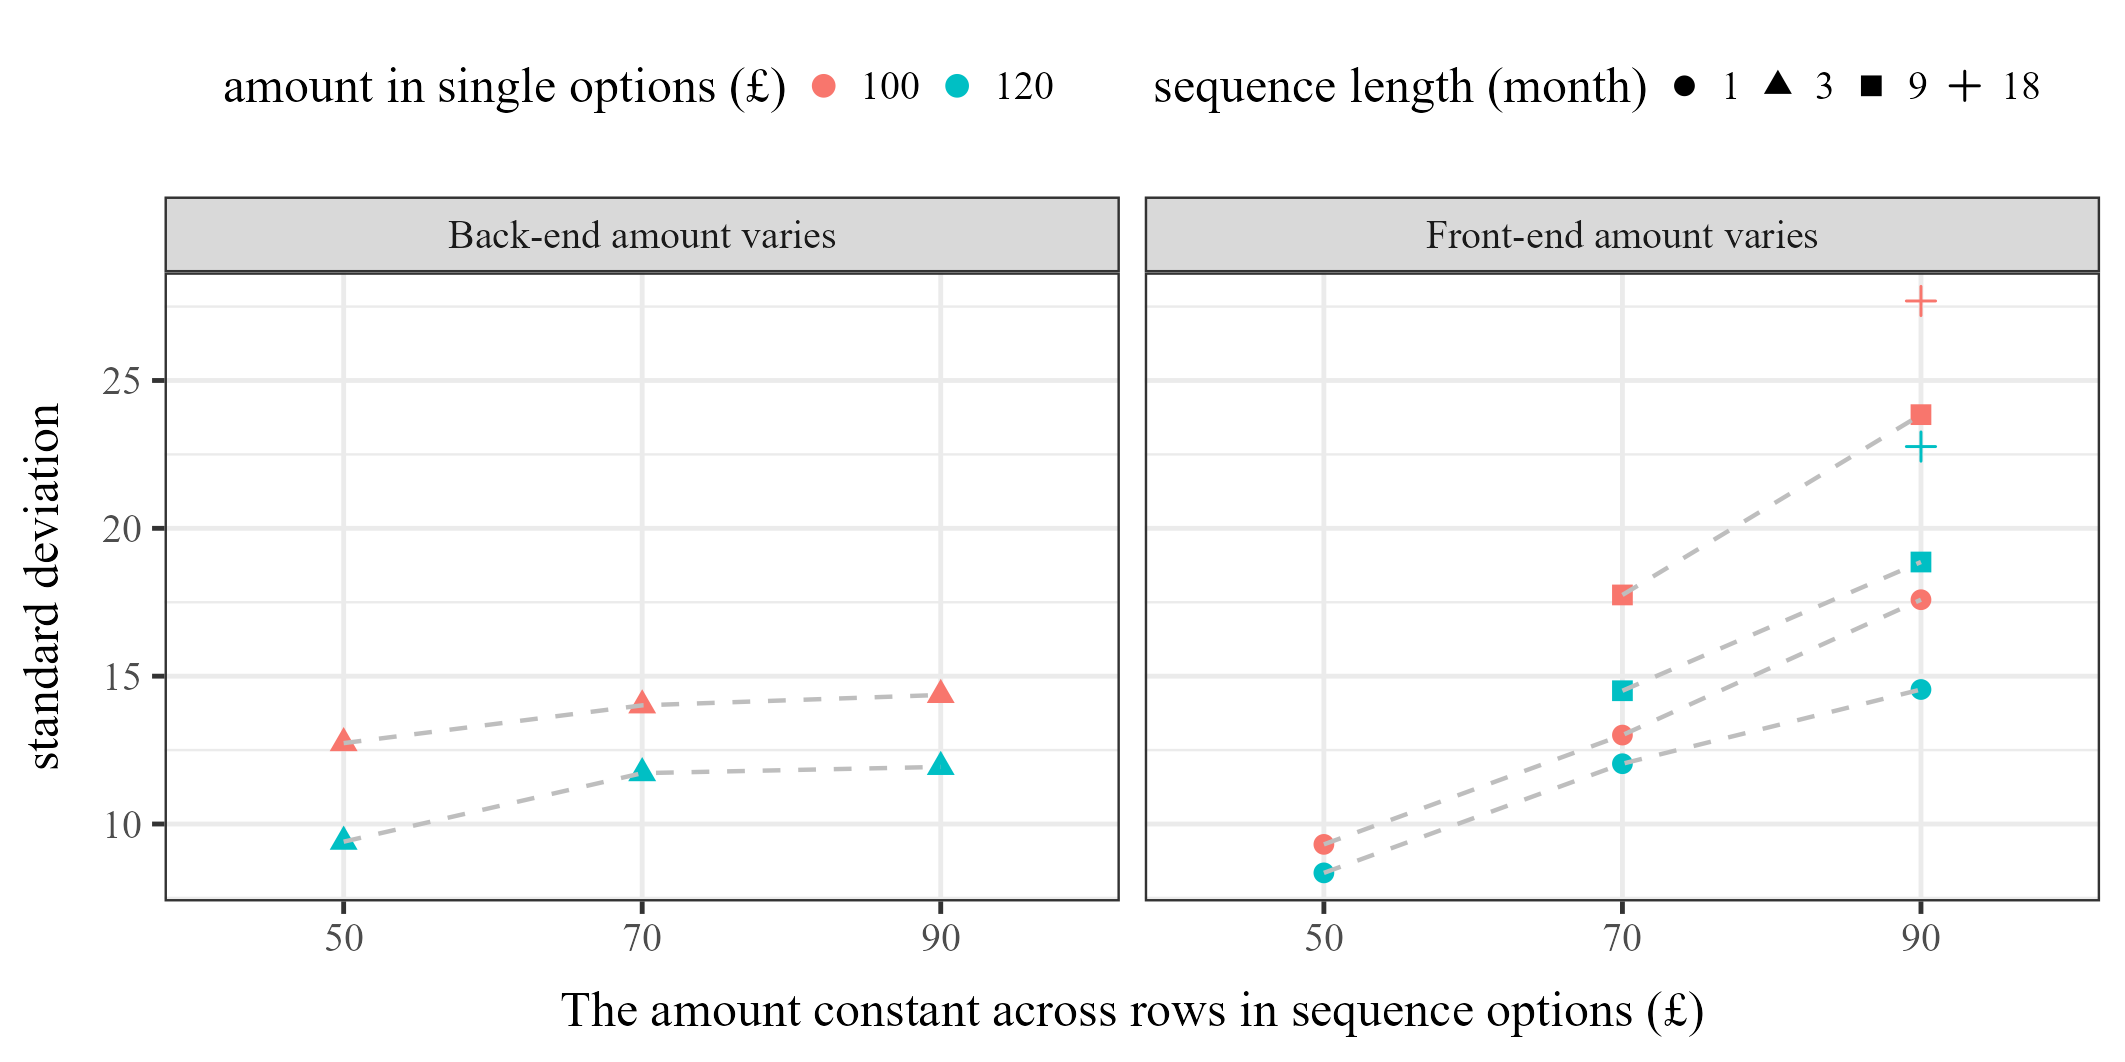
\includegraphics[width=0.96\textwidth]{figures/exp1_indiff_point_sd.png}   
  \caption{Standard deviation of indifference points in Experiment 3}      
  \label{fig:exp1_indiff_sd} 
\end{figure}

The standard deviation of indifference points provides a measure for
participants' sensitivity to the amount varying across rows in each
question. A smaller variance indicates a greater sensitivity of choice
to changes in that amount. To illustrate, one can imagine an extreme
case. Suppose all participants prefer ``receive £100 today'' (single
option) to ``receive £50 today and £70 in 1 month'' (sequence option) in
a question, but on the next row where the front-end amount increases
from £50 to £60, they all prefer the sequence option. Then, all of their
indifference point will be £55 and there is no variance in their
choices. In other words, they are extremely sensitive to this change in
the front-end amount so that it increases their likelihood of choosing
the sequence option by 100\%. By contrast, each change in that amount
only increases the likelihood by a small level, we should observe a
great variance in their choices.

The right side of Figure \ref{fig:exp1_indiff_sd} indicates, keeping the
others equal, in the ``front-end amount varies'' condition, either
increasing the back-end amount or delaying the delivering of this amount
would result in a greater standard variance. Meanwhile, the left side of
Figure \ref{fig:exp1_indiff_sd} indicates, in the ``back-end amount
varies'' condition, increasing the front-end amount also results in a
greater standard variance in indifference points. All these implies that
when valuing the sequence options, people are less sensitive to changes
in an amount if the other amount gets larger, and they are less
sensitive to changes in the front-end amount if delay of the back-end
amount gets longer.

\hypertarget{model-estimation}{%
\subsubsection{Model Estimation}\label{model-estimation}}

For regression analysis, we draw the insights from Section
\ref{impli_prob_choice} and construct a probabilistic choice model. Let
``receive \(M\) today'' denote the single option and ``receive \(X_1\)
today and \(X_T\) in delay \(T\)'' denote the sequence option for any
specific choice. Each condition is analyzed separately. In the
``front-end amount varies'' condition, only \(X_1\) is varying across
rows within each question. So, we focus on the variation of \(w_1\) with
other variables. Similarly, in the ``back-end amount varies'' condition,
we only focus on \(w_T\).

In each condition, let \(X_c\) denote the amount constant in the
sequence options, \(X_v\) denote the amount varying across rows.
Assuming the weights are independent of other variables, we can
generalize Equation (2) by\[ P = \phi(w\cdot u(X_v)+g(M,X_c,T)) \]where
\(w\cdot u(X_v)\) represents \(w_1\cdot u(X_1)\) in the ``front-end
amount varies'' condition and represents \(w_T\cdot u(X_T)\) in the
``back-end amount varies'' condition, and \(g(M,X_c,T)\) represents all
the other terms in Equation (2). We allow \(g(M,X_c,T)\) to be a
non-linear term. To construct it, we create a dummy variable for each
question (each question has a unique combination of \(M\), \(X_c\) and
\(T\)) and take these dummies as random intercepts. We transfer \(M\),
\(X_c\), and \(T\) to dummy variables, and set their minimum levels as
the control levels. To examine how the coefficient of \(u(X_v)\) would
be affected by other variables, we construct the interactions between it
and each level of \(X_c\), \(M\) and \(T\).

The link function is set to be \(\phi(v)=1/(1+e^{-v})\). In other words,
we predict participants' choices with logistic regressions. Following
\citet{andersen2008eliciting}, we consider a concave utility function
\(u(x)=(\omega+x)^\gamma\), \(0<\gamma<1\), \(\omega\geq0\), where
\(\gamma\) denotes the risk aversion coefficient and \(\omega\) denotes
background consumption. To estimate \(\gamma\) and \(\omega\), we
construct a probabilistic choice model and fit it with the data from
risky choice questions. Appendix C provides more details about the
estimation method. As a result, we obtain \(\gamma=0.695\) and
\(\omega\approx 0.000\) .\footnote{In Table \ref{tab:exp1_reg_baseline}
  of the Appendix, we also report the estimates obtained under
  risk-neutral utility function \(u(x)=x\). The results suggest
  considering a concave utility function improves the goodness of fit
  (producing to a lower AIC).}

We report the model estimation results in Table
\ref{tab:exp1_reg_utility}. Each model is fitted with the maximum
likelihood method. Column (1) and (3) reports the results of pooled
regressions, and Column (2) and (4) report the results of the models
including participant-specific dummies as random intercepts. In general,
the results suggest either a large \(X_c\) or a longer \(T\) can reduce
the coefficient \(w\) in Equation (3).\footnote{In Table
  \ref{tab:exp1_reg_censor} of the Appendix, we remove the rows where
  all participants choose the same option and then run the same
  regressions. These results are still valid.} For the ``front-end
amount varies'' condition, increasing the back-end amount from the
lowest level £50 to its middle level \(X_{mid}\) and highest level
\(X_{high}\) (which is £70 and £90 respectively) could reduce the
coefficient of \(u(X_v)\), i.e. \(w_1\), by 0.502 and 0.833 according to
Column (2), with \(p=0.021\) for the former estimate and \(p<0.0001\)
for the latter estimate. Meanwhile, as the delay of the back-end amount
increases from its lowest level ``1 month'' to the middle level
\(T_{mid}\) ``9 months'', and to the highest level \(T_{high}\) ``18
months'', the coefficient of \(u(X_v)\) is reduced by 0.222 and 0.325
respectively, with \(p<0.0001\) for both estimates.

Under the ``back-end amount varies'' condition, note the back-end amount
is delivered in 3 months for each question. In this case, increasing the
front-end amount from the lowest level to its middle level \(X_{mid}\)
and highest level \(X_{high}\) could reduce the coefficient of
\(u(X_v)\), i.e. \(w_2\), by 0.284 and 0.501 according to Column (4),
with \(p=0.009\) for the former estimate and \(p<0.0001\) for the latter
estimate. This result is consistent with the behavior of a certain
proportion of participants in Experiment 2: they discount the value of
the back-end amount more when there is a larger front-end amount.


\documentclass[12pt]{article}


\begin{document}
\begin{table}
    \caption{Regression Results for Experiment 3}
    \vspace*{12pt}
    \centering

      \begin{tabular}{lllll}
\hline
 & \multicolumn{2}{r}{Front-end amount varies} & \multicolumn{2}{r}{Back-end amount varires} \\
 & (1) Pooled & (2) FE & (1) Pooled & (2) FE \\
\hline
$u(X_v)$ & 0.921$^{***}$ & 1.605$^{***}$ & 0.72$^{***}$ & 1.657$^{***}$ \\
 & (0.121) & (0.243) & (0.057) & (0.154) \\
$u(X_v)\cdot1\{M=M_{high}\}$ & 0.129$^{***}$ & 0.206$^{***}$ & 0.246$^{***}$ & 0.504$^{***}$ \\
 & (0.016) & (0.031) & (0.034) & (0.078) \\
$u(X_v)\cdot1\{X_c=X_{mid}\}$ & -0.294$^{*}$ & -0.502$^{*}$ & -0.141$^{***}$ & -0.284$^{**}$ \\
 & (0.12) & (0.217) & (0.045) & (0.109) \\
$u(X_v)\cdot1\{X_c=X_{high}\}$ & -0.498$^{***}$ & -0.833$^{***}$ & -0.257$^{***}$ & -0.501$^{***}$ \\
 & (0.119) & (0.223) & (0.046) & (0.109) \\
$u(X_v)\cdot1\{T=T_{mid}\}$ & -0.129$^{***}$ & -0.222$^{***}$ &  &  \\
 & (0.029) & (0.048) &  &  \\
$u(X_v)\cdot1\{T=T_{high}\}$ & -0.181$^{***}$ & -0.325$^{***}$ &  &  \\
 & (0.037) & (0.06) &  &  \\\hline

observations & 18840 & 18840 & 9420 & 9420 \\
AIC & 11310.724 & 6824.27 & 4150.095 & 2099.21 \\
\hline
\end{tabular}
% INSERT exp1_utility_model

    \vspace*{4pt}
    \centering
    \begin{minipage}{0.85\textwidth}
    {\par\footnotesize Note: * $p<0.05$, ** $p<0.01$, *** $p<0.005$. Standard errors are clustered at the subject level and are reported in the parentheses. The $p$-values are calculated based on Wald tests. $X_c$ denotes the amount constant in a choice list, and its middle and highest levels are $X_{mid}$ and $X_{high}$. $T$ denotes the delay of the back-end amount, and its middle and highest levels are $T_{mid}$ and $T_{high}$. $M$ denotes amount in the single option, and its higher level is $M_{high}$. $X_v$ denotes the amount varying across rows. The utility function is $u(x)=x^{0.695}$.  Every model includes question-specific dummies as random intercepts. Column (2) and (4) come from a model including participant-specific dummies as random intercepts.}
    \end{minipage}
    \label{tab:exp1_reg_utility}
\end{table}

\end{document}



Our results also suggest an increase in \(M\), i.e.~the amount in single
option, would increase the participants' sensitivity to the amount
varying across rows. In Figure \ref{fig:exp1_indiff_sd}, the
indifference points have a smaller variance under the higher level of
\(M\) (which is £120). In Table \ref{tab:exp1_reg_utility}, the
coefficient of \(u(X_v)\) is significantly increased when
\(M=M_{high}\), with \(p<0.0001\) for each column. This indicates the
reference points may also have an effect on time discounting. A relevant
evidence to this might be the magnitude effect, i.e.~people exhibit more
patience in choices between larger amounts. To illustrate, suppose the
front-end amount in each question is always 0 and thus the choice is
between receiving \(M\) today and receiving \(X_v\) later. If we assume
the utility of each amount is determined by our estimated utility
function, the magnitude effect would predict that an increase in \(M\)
from £100 to £120 can result in \(u(X_v)\) being less discounted
\citep{andersen2013discounting}. This exactly implies the coefficient of
\(u(X_v)\) in our analytic framework should be increasing with \(M\).

\hypertarget{discussion}{%
\section{Discussion}\label{discussion}}

In this section, we discus the relationship between the results of
Experiment 1-3 and some theories about time discounting. In Experiment
1, we exogenously manipulate attention and find this effectively alters
participants' time preferences. In Experiment 2, a substantial portion
of participants valuate any reward sequence simply by its total money.
To the best of our knowledge, both results cannot be accounted for by
the existing time discounting theories.

In Experiment 2-3, we also find evidence supporting our arguments about
(in-)attention to small values. In Experiment 2, we find when people
valuate a sequence of two positive rewards, an increase in the front-end
amount could make (some of) them discount the value of the back-end
amount more. In Experiment 3, our model estimation results suggest an
increase in one reward or in sequence length could make the total value
of sequence less sensitive to another reward, which may indicate people
discount the value of the another reward more. These results can be
(partially) generated by certain theories related to attention.

First, the salience theory
\citep{bordalo2012salience, bordalo2013salience} proposes that a reward
stimulus would look more salient if it differs more greatly from a
reference point. When people valuate a reward sequence, they tend to
overweight the salient rewards and underweight the non-salient rewards.
Taking zero as the reference point, when there is a large reward in the
sequence, the salience theory would predict that it can attract much
attention and therefore reduce the weights assigned to other rewards,
i.e.~making them more discounted. Nevetheless, the salience theory
cannot account for the hidden-zero effect and our finding that a longer
delay of the back-end amount could make the value of the front-end
amount more discounted. To incorporate such evidence, adding zero values
into the sequence should reduce the ``salience'' of positive rewards.
This may require us to add an extra constraint on the total volume of
weights. For example, fixing the sum of weights at a certain level so
that allocating weights to new zero values would definitely reduce the
weights for other rewards.

Second, \citet{noor2022optimal,noor2024constrained} propose a theory
related to optimal allocation of attention across time points. In their
theory, decision makers originally focus on the current time, but to
process a reward sequence, they should allocate attention weights to
future times, which incurs a cognitive cost. The decision makers'
objective is to maximize the total value of the sequence minus the
incurred cognitive cost. Their theory also predicts that people tend to
assign greater weights to larger rewards. Under certain cognitive cost
functions and constraints, the theory can produce the results of our
experiments.

Apart from attention theories, there are also other theories that can
explain some of our results. For example, the intertemporal trade-off
model
\citep{read2012tradeoffs, scholten2016cumulative, scholten2024unified}
proposes that when valuating a reward sequence, people would value the
amounts and the times separately. The total value of the sequence is the
utility of the total money minus a delay cost. Increasing an earlier
amount in the sequence can reduce the delay cost, while increasing a
later amount can increase the delay cost. According to the most recent
version of this model, for sequence options in our experiments, a large
back-end amount would make each unit increase in the front-end amount
reduces the delay cost by a greater degree, and a large front-end amount
would make each unit increase in the back-end amount increases the delay
cost by a smaller degree. Meanwhile, in either case, the utility of
total money should increase by a smaller degree due to the concavity of
utility function. When the latter effect exceeds the former effect, a
large reward can make the total value less sensitive to the other
amount. However, under a longer delay of the back-end amount, increasing
the front-end amount should reduce the delay cost by a greater degree.
Therefore, under this circumstance, the intertemporal trade-off model
predicts people are more sensitive to the front-end amount, while the
results of Experiment 3 indicate the reverse.

\renewcommand\refname{References}
  \bibliography{reference.bib}

\newpage
\renewcommand\thefigure{B.\arabic{figure}}    
\setcounter{figure}{0}

\renewcommand\thetable{A.\arabic{table}}    
\setcounter{table}{0}

\hypertarget{appendix}{%
\section*{Appendix}\label{appendix}}
\addcontentsline{toc}{section}{Appendix}

\hypertarget{a.-additional-tables}{%
\subsection*{A. Additional Tables}\label{a.-additional-tables}}
\addcontentsline{toc}{subsection}{A. Additional Tables}


\begin{table}[!h]
    \caption{Predicting response times with choices and conditions in Experiment 1}
    \vspace*{10pt}
    \centering

      \begin{tabular}{lll}
\hline
 & Intertemporal Choice & Count-the-Rabbits \\
\hline
Group & -0.684$^{***}$ & -0.792$^{***}$ \\
 & (0.141) & (0.144) \\
Question$\cdot1\{\text{Group}=0\}$ & -0.165 & 0.912$^{***}$ \\
 & (0.174) & (0.199) \\
Question$\cdot1\{\text{Group}=1\}$ & 0.457$^{***}$ & 0.849$^{***}$ \\
 & (0.101) & (0.132) \\
Choice & 0.954$^{*}$ & 1.291$^{***}$ \\
 & (0.399) & (0.456) \\
Choice$\times$Group & -0.762$^{*}$ & -1.265$^{***}$ \\
 & (0.304) & (0.229) \\
Choice$\times$Question$\cdot1\{\text{Group}=0\}$ & 0.001 & -0.138 \\
 & (0.257) & (0.23) \\
Choice$\times$Question$\cdot1\{\text{Group}=1\}$ & -0.12 & 0.263 \\
 & (0.195) & (0.175) \\\hline

observations & 4393 & 2179 \\
AIC & 18560.034 & 8711.872 \\
adj-$R^2$ & 0.381 & 0.55 \\
\hline
\end{tabular}
% INSERT reg_response_time

    \vspace*{4pt}
    \centering
    \begin{minipage}{0.85\textwidth}
    {\par\footnotesize Note: * $p<0.05$, ** $p<0.01$, *** $p<0.005$. Both models are estimated through 2SLS method. For first-stage regression, we use the model for Column (2) in Table \ref{tab:exp3_reg_intertemporal_choice} to predict intertemporal choices, and the model for Column (3) in Table \ref{tab:exp3_reg_rabbit_choice} to predict count-the-rabbits choices. The variable Choice which is 1 if the predicted choice is the sequence option and is 0 otherwise. For second-stage regression, indepdent variables are the predictors shown in the table plus task-specific dummies and their interactions with Choice, and participant-specific dummies. Standard errors (in the parentheses) are clustered at the subject level. $p$-values are calculated based on t-tests. }
    \end{minipage}
    \label{tab:exp3_reg_response_time}
\end{table}





\documentclass[12pt]{article}


\begin{document}
\begin{table}
    \caption{Regression results with risk-neutral utility function for Experiment 3}
    \vspace*{12pt}
    \centering

      \begin{tabular}{lllll}
\hline
 & \multicolumn{2}{r}{Front-end amount varies} & \multicolumn{2}{r}{Back-end amount varires} \\
 & (1) Pooled & (2) FE & (1) Pooled & (2) FE \\
\hline
$X_v$ & 0.181 & 0.316$^{***}$ & 0.139$^{***}$ & 0.318$^{***}$ \\
 & (0.339) & (0.044) & (0.011) & (0.03) \\
$X_v\cdot1\{M=M_{high}\}$ & 0.022$^{***}$ & 0.031$^{***}$ & 0.039$^{***}$ & 0.071$^{***}$ \\
 & (0.006) & (0.006) & (0.007) & (0.017) \\
$X_v\cdot1\{X_c=X_{mid}\}$ & -0.047 & -0.079$^{*}$ & -0.015 & -0.024 \\
 & (0.032) & (0.04) & (0.009) & (0.023) \\
$X_v\cdot1\{X_c=X_{high}\}$ & -0.083$^{**}$ & -0.135$^{***}$ & -0.026$^{**}$ & -0.031 \\
 & (0.031) & (0.041) & (0.01) & (0.023) \\
$X_v\cdot1\{T=T_{mid}\}$ & -0.033$^{***}$ & -0.058$^{***}$ &  &  \\
 & (0.006) & (0.012) &  &  \\
$X_v\cdot1\{T=T_{high}\}$ & -0.046$^{***}$ & -0.085$^{***}$ &  &  \\
 & (0.012) & (0.015) &  &  \\\hline

observations & 18840 & 18840 & 9420 & 9420 \\
AIC & 11455.38 & 6963.578 & 4215.293 & 2158.83 \\
\hline
\end{tabular}
% INSERT exp1_baseline_model

    \vspace*{4pt}
    \centering
    \begin{minipage}{0.85\textwidth}
    {\par\footnotesize Note: * $p<0.05$, ** $p<0.01$, *** $p<0.005$. Standard errors are clustered at the subject level and are reported in the parentheses. The $p$-values are calculated based on Wald tests. $X_c$ denotes the amount constant in a choice list, and its middle and highest levels are $X_{mid}$ and $X_{high}$. $T$ denotes the delay of the back-end amount, and its middle and highest levels are $T_{mid}$ and $T_{high}$. $M$ denotes amount in the single option, and its higher level is $M_{high}$. $X_v$ denotes the amount varying across rows. Every model includes question-specific dummies as random intercepts. Column (2) and (4) come from a model including participant-specific dummies as random intercepts.}
    \end{minipage}
    \label{tab:exp1_reg_baseline}
\end{table}

\end{document}




\documentclass[12pt]{article}


\begin{document}
\begin{table}
    \caption{Regression results on the censored data in Experiment 3}
    \vspace*{12pt}
    \centering

      \begin{tabular}{lllll}
\hline
 & \multicolumn{2}{r}{Front-end amount varies} & \multicolumn{2}{r}{Back-end amount varires} \\
 & (1) Pooled & (2) FE & (1) Pooled & (2) FE \\
\hline
$u(X_v)$ & 0.914$^{**}$ & 1.584$^{***}$ & 0.712$^{***}$ & 1.65$^{***}$ \\
 & (0.342) & (0.247) & (0.059) & (0.155) \\
$u(X_v)\cdot1\{M=M_{high}\}$ & 0.107$^{*}$ & 0.193$^{***}$ & 0.187$^{***}$ & 0.484$^{***}$ \\
 & (0.053) & (0.03) & (0.037) & (0.08) \\
$u(X_v)\cdot1\{X_c=X_{mid}\}$ & -0.314$^{*}$ & -0.499$^{*}$ & -0.134$^{***}$ & -0.281$^{*}$ \\
 & (0.129) & (0.226) & (0.047) & (0.111) \\
$u(X_v)\cdot1\{X_c=X_{high}\}$ & -0.509$^{***}$ & -0.828$^{***}$ & -0.248$^{***}$ & -0.5$^{***}$ \\
 & (0.127) & (0.231) & (0.048) & (0.111) \\
$u(X_v)\cdot1\{T=T_{mid}\}$ & -0.115$^{***}$ & -0.212$^{***}$ &  &  \\
 & (0.03) & (0.049) &  &  \\
$u(X_v)\cdot1\{T=T_{high}\}$ & -0.163$^{***}$ & -0.312$^{***}$ &  &  \\
 & (0.036) & (0.061) &  &  \\\hline

observations & 14915 & 14915 & 6594 & 6594 \\
AIC & 11226.482 & 6797.682 & 4120.484 & 2094.364 \\
\hline
\end{tabular}
% INSERT exp1_utility_censor

    \vspace*{4pt}
    \centering
    \begin{minipage}{0.9\textwidth}
    {\par\footnotesize Note: * $p<0.05$, ** $p<0.01$, *** $p<0.005$. FE denotes a model including participant-specific dummies as random intercepts. Each model and the estimation method are the same as Table \ref{tab:exp1_reg_utility}. However, for each question, the rows where all participants choose the same option are removed from the sample. }
    \end{minipage}
    \label{tab:exp1_reg_censor}
\end{table}

\end{document}



\newpage

\hypertarget{b.-additional-figures}{%
\subsection*{B. Additional Figures}\label{b.-additional-figures}}
\addcontentsline{toc}{subsection}{B. Additional Figures}

\begin{figure}
  \centering
  \begin{subfigure}{\textwidth}
    \centering
    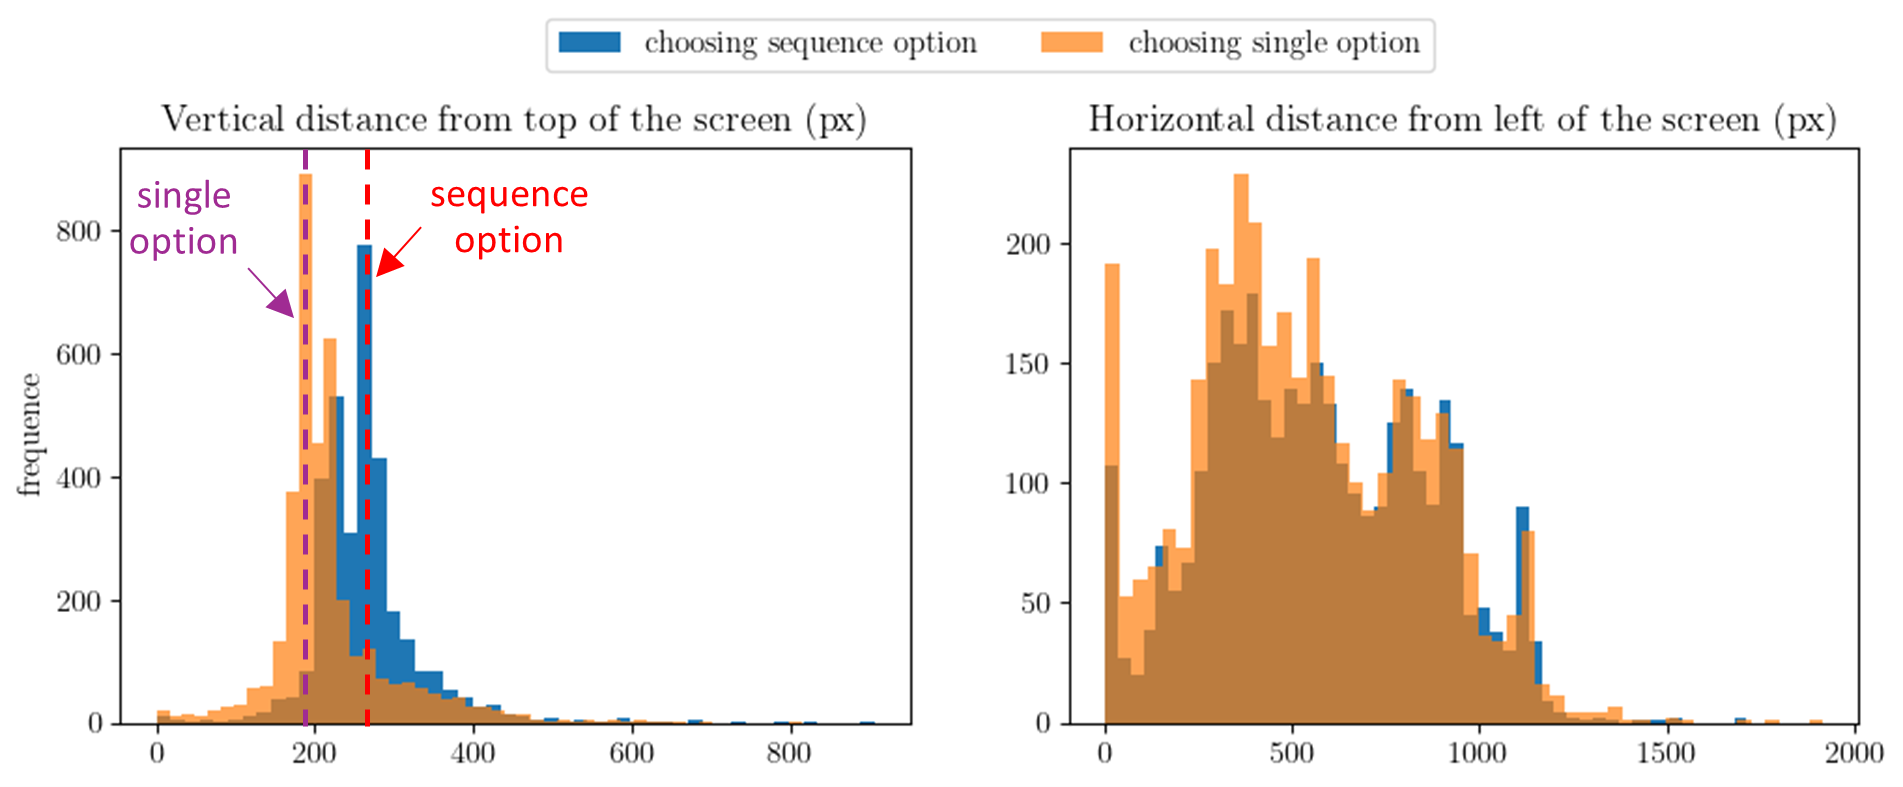
\includegraphics[width=\linewidth]{figures/exp3_mouse_intertemporal.png}
    \subcaption{Intertemporal Choice Task}
  \end{subfigure}
  \begin{subfigure}{\textwidth}
    \vspace{1.5em}
    \centering
    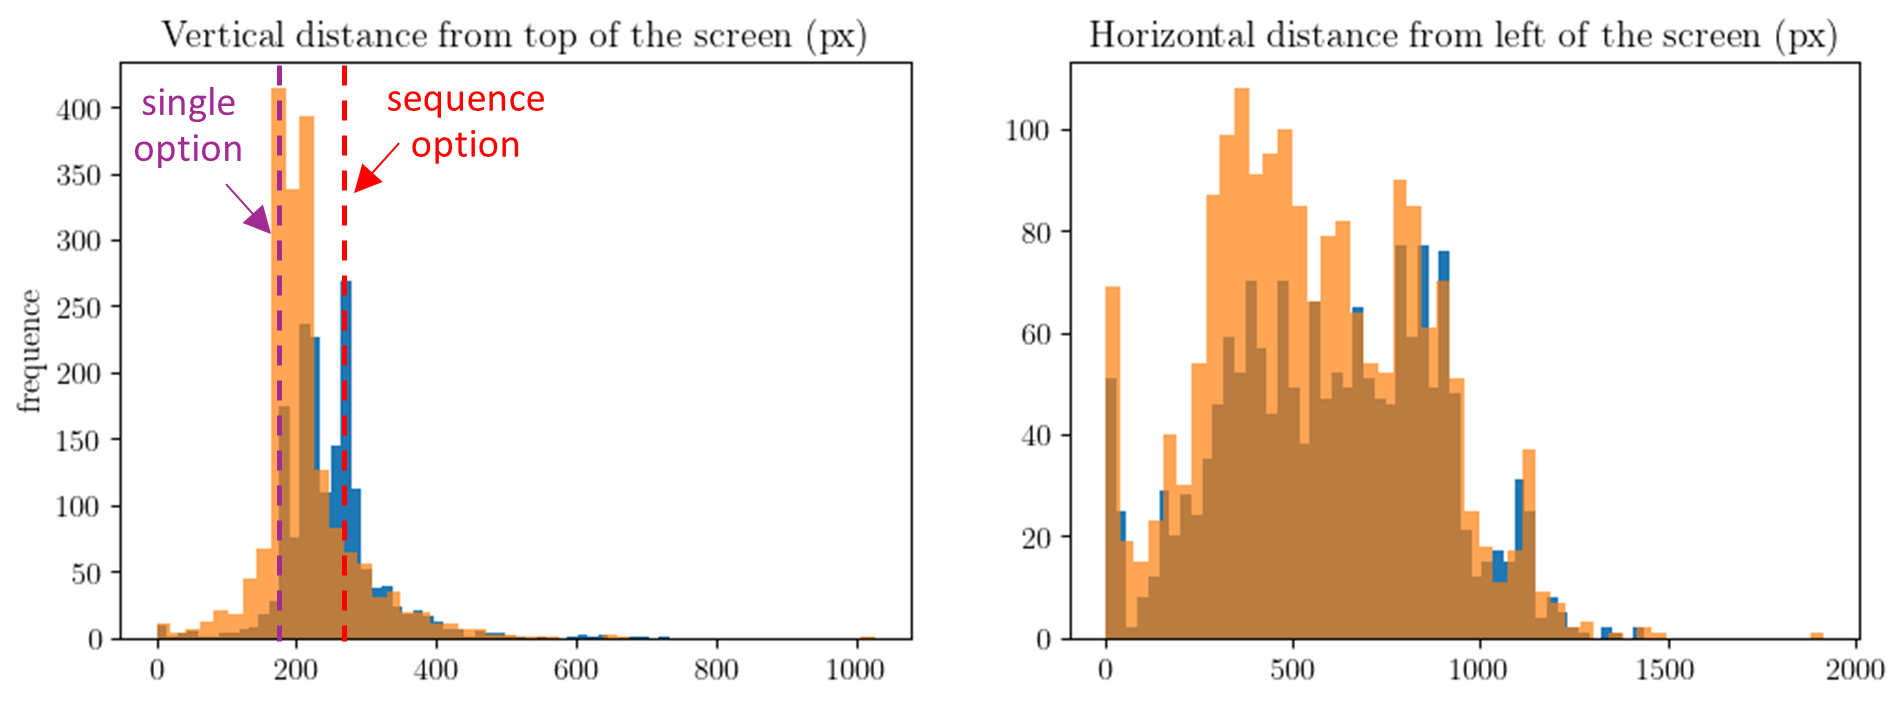
\includegraphics[width=\linewidth]{figures/exp3_mouse_rabbit.png}
    \subcaption{Count-the-Rabbits Task}
  \end{subfigure}
  \caption{Mouse positions recorded at the end of the forced viewing period}
  \label{fig:exp3_mouse_position}
\end{figure}

\begin{figure} 
\centering
\begin{subfigure}{0.85\textwidth}
  \hfill
  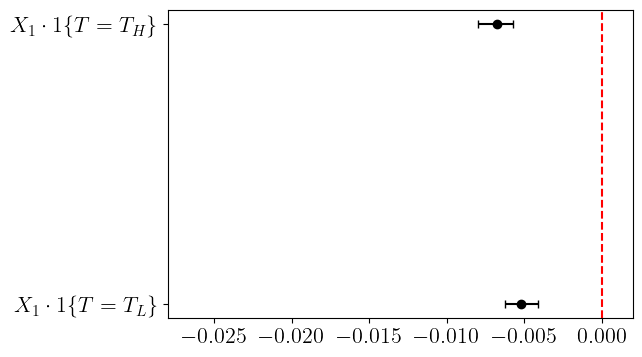
\includegraphics[width=0.85\linewidth]{figures/exp2_bootstrap_ci_baseline.png}
\end{subfigure}
\begin{subfigure}{0.85\textwidth} 
  \hfill
  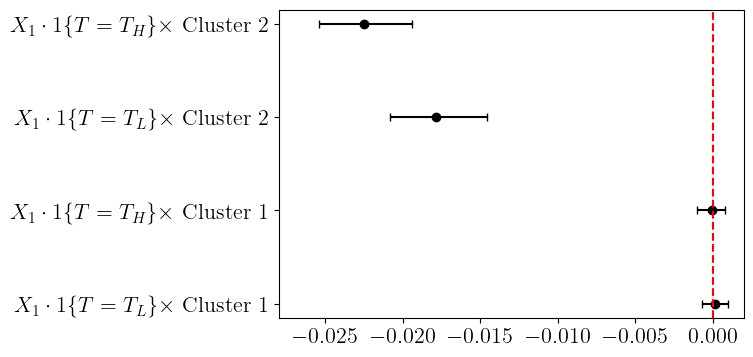
\includegraphics[width=\linewidth]{figures/exp2_bootstrap_ci_label.png} 
\end{subfigure}
\caption{Bootstrap 95\% confidence intervals for coefficients in the robust regressions}
\vspace*{4pt}
\centering

\begin{minipage}{1.0\textwidth}
{\par\footnotesize Note: The subfigures on the top and the bottom correspond to Column (5) and (6) in Table \ref{tab:exp2_seq_value_reg} respectively. The dots are the original estimates and the error bars indicate the confidence intervals. To approximate the distribution for each coefficient, we use the stratified bootstrap method. The observations are divided into three strata based on RLM results: the upper tail (with high residuals and a weight of 1), the lower tail (with low residuals and a weight of 1), and the others. We draw observations with replacement within each stratum and use them to estimate the coefficients. Each bootstrap sample is the same size as the original sample, and the process is repeated 1,000 times. }
\end{minipage}
\label{fig:exp2_bootstrap_ci}
\end{figure}

\begin{figure} 
\centering
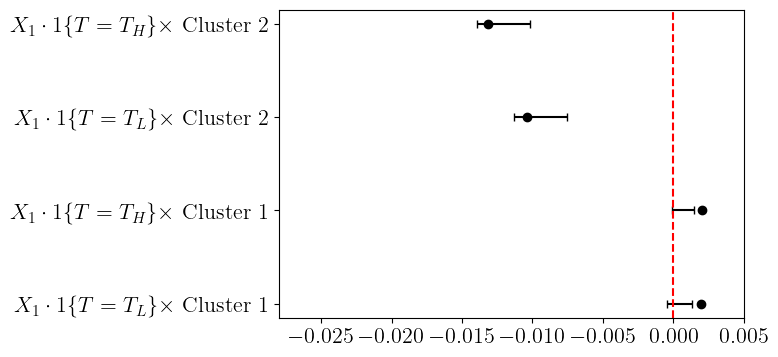
\includegraphics[width=0.85\linewidth]{figures/exp2_bootstrap_ci_label_gmm_fe.png}
\caption{Regression coefficients - using Gaussian mixture model for clustering}
\vspace*{4pt}
\centering

\begin{minipage}{1.0\textwidth}
{\par\footnotesize Note: The regression model is the same as Column (6) in Table \ref{tab:exp2_seq_value_reg}. Estimation method is the same as Figure \ref{fig:exp2_bootstrap_ci}. The dots are the original estimates and the error bars indicate the boostrap 95\% confidence intervals. }
\end{minipage}
\label{fig:exp2_bootstrap_ci_gmm}
\end{figure}

\newpage

\hypertarget{c.-method-to-estimate-risk-aversion-coefficient}{%
\subsection*{C. Method to estimate risk aversion
coefficient}\label{c.-method-to-estimate-risk-aversion-coefficient}}
\addcontentsline{toc}{subsection}{C. Method to estimate risk aversion
coefficient}

For any risky choice \(i\), let ``get \(X_i^R\) with a 50\% chance''
denote the risky option and ``get \(X_i^S\) with certainty'' denote the
safe option. Note \(X_i^R\) is constant within a choice list while
\(X_i^S\) is varying across rows. Assume that participants choose the
safe option with probability \(P_i^{\text{risk}}\), and\[
P_i^{\text{risk}} = \frac{1}{1+e^{-\frac{\Delta U}{\lambda}}}
\]where \(\Delta U = u(X_i^S) - 0.5\cdot u(X_i^R)\) and \(\lambda\)
(\(\lambda >0\)) is a temperature parameter that controls the randomness
of choice. The utility function is \(u(x)=(\omega+x)^\gamma\),
\(0<\gamma<1\), \(\omega\geq 0\). We fit the model with the maximum
likelihood method. The log-likelihood function is\[
LL(\gamma,\lambda) = \sum_{i=1}^N \xi_i\ln(P_i^{\text{risk}})+(1-\xi_i)\ln(1-P_i^{\text{risk}}) 
\]We use \(\gamma=1\), \(\lambda =1\) as the initial values and maximize
the log-likelihood function with the SLSQP algorithm. The model is
fitted on the 3,297 observations of the risky choices. In the solution,
\(LL=-1711.87\), \(\gamma=0.695\), \(\lambda=1.904\),
\(\omega\approx 2.245\times10^{-13}\).

\end{document}
